\documentclass[usenames,dvipsnames]{beamer}

% French characters
\usepackage[utf8x]{inputenc}
\usepackage[T1]{fontenc}
% French display
\usepackage[english]{babel}
% Math package
\usepackage{amsmath}
\usepackage{amsfonts}
\usepackage{amssymb}
% includegraphics
\usepackage{graphicx}
% units
%\usepackage{hepunits}
% links
\usepackage{hyperref}
% \usepackage[bookmarksopen,bookmarksopenlevel=1]{hyperref}
\usepackage{colortbl}
\usepackage{tikz}
\usepackage{rotating}
% Theme & Color theme
\usepackage{default}
\usetheme{Frankfurt}
\usecolortheme{perso}
% My green
\definecolor{MyColor}{RGB}{43,153,43}
\setbeamercolor{structure}{fg=MyColor}
\setbeamertemplate{title page}[default]
\setbeamercolor{title}{bg=}

% \setbeamercolor{titlelike}{fg=MyColor}
% \setbeamercolor{palette primary}{fg=MyColor}
% \setbeamercolor{palette secondary}{fg=MyColor}
% \setbeamercolor{palette tertiary}{bg=MyColor}
% \setbeamercolor{palette quaternary}{bg=MyColor}
% Font
\usepackage{times}
\usefonttheme[onlymath]{serif}
% Suppress the navigation bar
% \beamertemplatenavigationsymbolsempty
\setbeamertemplate{navigation symbols}{}

% Outerthemes
% \useoutertheme[footline=empty, subsection=false]{miniframes}
% \useoutertheme[subsection=false]{miniframes}
% \useoutertheme[subsection=false]{smoothbars}
% gets rid of bottom navigation bars
\setbeamertemplate{footline}[page number]{}
% 
% \setbeamercolor{frametitle}{parent=palette primary}
% \setbeamercolor{subsection in head/foot}{parent=palette secondary}
% \setbeamercolor{section in head}{parent=palette quaternary}
% \setbeamercolor{section in sidebar}{fg=black}
% \setbeamercolor{section in sidebar shaded}{fg= grey}
% Appendix page numbering
\usepackage{appendixnumberbeamer}
% feynmp for Feynman diagrams
%\usepackage{feynmp}
%\DeclareGraphicsRule{*}{mps}{*}{}
\makeatletter
\def\endfmffile{%
  \fmfcmd{\p@rcent\space the end.^^J%
          end.^^J%
          endinput;}%
  \if@fmfio
    \immediate\closeout\@outfmf
  \fi
  \ifnum\pdfshellescape=\@ne
    \immediate\write18{mpost \thefmffile}%
  \fi}
\makeatother
\usepackage[abs]{overpic}
\def\met{\ensuremath{\not\!\!{E_{T}}}}

\newcommand{\ttbar}{$t\bar{t}$}
\newcommand{\bbbar}{$b\bar{b}$}
\newcommand{\GeVcc}{GeV/$\text{c}^2$}
\newcommand{\pt}{$p_{T}$}
\newcommand{\ptg}[1]{$p_{T}>#1$~GeV/c}
\newcommand{\etal}[1]{$|\eta|<#1$}
\newcommand{\etag}[1]{$|\eta|>#1$}
\newcommand{\HT}{$H_{T}$}
\newcommand{\MET}{$\slashed{E}_{T}$}
\newcommand{\METg}[1]{$\slashed{E}_{T}>#1$~GeV/c}
\newcommand{\HTg}[1]{${H_{T}>#1}$~GeV/c}
\newcommand{\jn}[1]{$j_{#1}$}
\newcommand{\ex}[1]{\times 10^{#1}}
\newcommand{\Z}{$Z^{0}$}
\newcommand{\tq}{$t$}
\newcommand{\W}{$W^{+/-}$}
\newcommand{\Hb}{$H^{0}$}
\newcommand{\Tp}{$T'$}
\newcommand{\Tj}{$T'j$}
\newcommand{\Tjj}{$T'jj$}

%% Title and such
\title{\texorpdfstring{Search for a vector-like quark \Tp~decaying \\into top+Higgs in single production mode \\in full hadronic final state using \\CMS data collected at 8 TeV\\}}
%\title{\texorpdfstring{Recherche d'un quark vectoriel \Tp~\\qui se desintegre en top+Higgs dans \\le mode de production célibataire \\dans le état final hadronique avec \\les données recollectées par l'éxperience CMS à 8 TeV\\}}
% \subtitle{
% }
\author[J.~Ruiz-\'{A}lvarez]{Jos\'{e} D. Ruiz-\'{A}lvarez}
\institute[IPN Lyon]{
% Institut de Physique Nucléaire de Lyon / Université Claude Bernard Lyon 1\\
\includegraphics[height=.6cm]{../Prelude/CNRS.png}\hspace{.5cm}

\includegraphics[height=.6cm]{udl.png}\hspace{.5cm}
\includegraphics[height=.6cm]{../Prelude/UCBL.png}\hspace{.5cm}
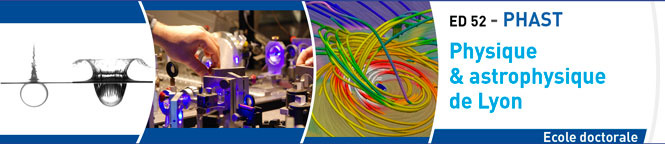
\includegraphics[height=.6cm]{EDPhast.jpg}
\\\vspace{.5cm}
\includegraphics[height=.7cm]{../Prelude/IPNL.png}\hspace{.5cm}
\includegraphics[height=.7cm]{../Prelude/CMS.png}
}
\date{21 octobre 2015}

% \mode<presentation> {
%   \usefonttheme{serif}
%   \useoutertheme[footline=authorinstitutetitle,subsection=false]{miniframes}
%   \usecolortheme{crane}
%   \useinnertheme[<shadow>]{rounded}
% }

% \setbeamercolor{boum}{bg=\color{white!40}, fg=black}
% 
% \addtobeamertemplate{block begin}{\pgfsetfillopacity{0.65}}{\pgfsetfillopacity{1}}
% 
% \newenvironment<>{varblock}[2][\textwidth]{%
%   \setlength{\textwidth}{#1}
%   \begin{actionenv}#3%
%     \def\insertblocktitle{#2}%
%     \par%
%     \usebeamertemplate{block begin}}
%   {\par%
%     \usebeamertemplate{block end}%
%   \end{actionenv}}
% 

\usepackage{fancybox}
\usepackage{framed,xcolor}
\colorlet{shadecolor}{white!60}
\usepackage{rotating}
% \usepackage[table]{xcolor} 

% \includeonly{11_StandardModel}
% \includeonly{11_StandardModel,12_LHC_CMS}
% \includeonly{12_LHC_CMS}
% \includeonly{11_StandardModel,12_LHC_CMS,13_Zgamma}
% \includeonly{13_Zgamma}
% \includeonly{14_Hgg,15_BSM}
% \includeonly{14_Hgg,BB_Hgg}
% \includeonly{13_Zgamma,14_Hgg,BB_Hgg}
% \includeonly{15_BSM,BB_BSM}
% \includeonly{BB_Zgamma}


\begin{document}

\begin{frame}[plain]
  \tikz[remember picture,overlay]
    \node (b) at
      (current page.center) [inner sep=0pt,opacity=.4]
%       (0.5\paperwidth,-0.5\paperheight) [inner sep=0pt,opacity=.4]
      {\begin{overpic}[height=.9\paperheight]{a-1_16_1_RhoPhi.png}\end{overpic}};
  \titlepage
\end{frame}

\setcounter{tocdepth}{1}
\begin{frame}{Plan}
\tableofcontents
\end{frame}


%%%%%%%%%%%%%%%%%%%%%%%%%%%%%%%%%%%%%%%%%%%%%%%%%%%%%%%%
%%%%%%%%%%%%%%%%%%%%%%%%%%%%%%%%%%%%%%%%%%%%%%%%%%%%%%%%
\section[Theory]{The Standard Model and beyond}
\setcounter{tocdepth}{2}

\begin{frame}
\begin{center}
The Standard Model and beyond
\end{center}
\end{frame}

\subsection{Theory}
\begin{frame}{The Standard Model}
\vspace{-.2cm}
\begin{columns}

\begin{column}{.50\textwidth}
\begin{block}{}
\begin{itemize}\scriptsize
%\item Theory developed from quantum theory and special relativity -> Quantum Field Theory (Feynman, Dirac, ...) + Continuous group symmetries (Noether, Yang, ...)
\item Model developed from quantum theory and special relativity $\to$ Quantum Field Theory + Continuous group symmetries
\item Fermions: matter components (electron, muon, quarks...)
\item Bosons: interaction mediators (\W, \Z, ...)
\item Extremely successful model: \\ quarks, CKM, \W~and \Z~masses, ...
\item But it is limited:
  \begin{itemize}\scriptsize
  \item Neutrino masses
  \item Dark matter
  \item \textbf{Hierarchy problem}
  \end{itemize}
\end{itemize}
\end{block}
\end{column}

\begin{column}{.50\textwidth}
\begin{figure}[!Hhtbp]
  \begin{center}
    \includegraphics[width=1.0\textwidth]{Standard_Model_of_Elementary_Particles.jpg}\\
    \vspace{.6cm}
    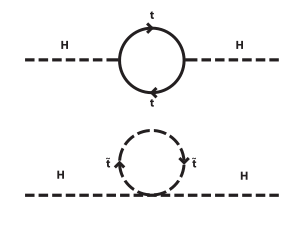
\includegraphics[width=0.8\textwidth]{SUSY.png}
    %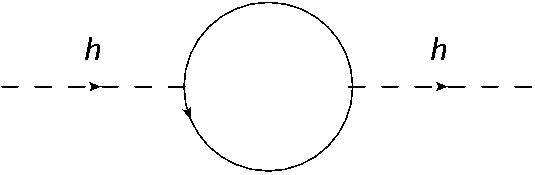
\includegraphics[width=0.8\textwidth]{../figs/HierarchyLoop.png}
    %\caption{Particle content of the standard model.}
    %\label{fig:SMContent}
  \end{center}
\end{figure}
\end{column}
\end{columns}
\end{frame}


\begin{frame}{Vector Like Quarks (VLQ)}
\vspace{-.3cm}
\begin{columns}

\begin{column}{.40\textwidth}
\begin{block}{}
\begin{itemize}\scriptsize
\item Motivated by the hierarchy problem $\to$ New states to cancel loop contributions
\item SM + not chiral quarks
\item States:
  \begin{itemize}\scriptsize
  \item $X$ 5/3 e
  \item \textbf{\Tp~2/3 e (as the top)}
  \item $B$ -1/3 e (as the b)
  \item $Y$ -4/3 e
  \end{itemize}
%\item \textbf{Generically they can be mixed with the three SM-quark generations}
%\item Produced in pairs or in single production mode with a SM-quark
%\item $T'\to bW^{+/-}, tZ^{0}, tH^{0}$
\end{itemize}
\end{block}
\end{column}

\begin{column}{.60\textwidth}
%\begin{figure}[!Hhtbp]
%  \begin{center}
%    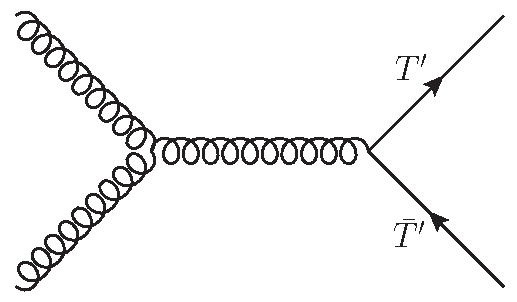
\includegraphics[width=0.5\textwidth]{../figs/Gluon_fusion_T_pair.jpg}
%    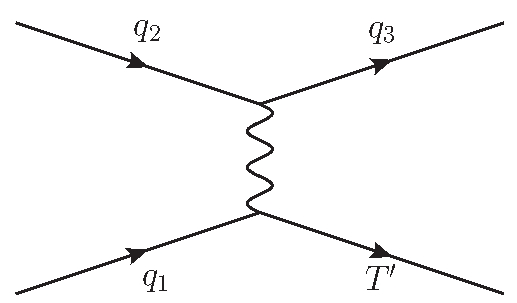
\includegraphics[width=0.5\textwidth]{../figs/Tchannel_T_single.jpg}
%  \end{center}
%\end{figure}
\tiny{
\begin{eqnarray}
  \mathcal{L}_{\binom{X}{T'}} & = & \kappa_{T}\left\{ \sqrt{\frac{\zeta_{i}\xi_{Z}^{T}}{\Gamma_{Z}^{0}}}\frac{g}{2c_{W}}\left[ \bar{T'}_{R}Z_{\mu}\gamma^{\mu}u^{i}_{R}\right]\right\} \nonumber\\
              & - & \kappa_{T}\left\{ \sqrt{\frac{\zeta_{i}\xi_{H}^{T}}{\Gamma_{H}^{0}}}\frac{M}{v}\left[ \bar{T'}_{L}Hu^{i}_{R}\right] + \sqrt{\frac{\zeta_{3}\xi_{H}^{T}}{\Gamma_{H}^{0}}}\frac{m_{t}}{v}\left[ \bar{T'}_{R}Ht_{L}\right]\right\} \nonumber\\            
              & + & \kappa_{X}\left\{ \sqrt{\frac{\zeta_{i}}{\Gamma_{W}^{0}}}\frac{g}{\sqrt{2}}\left[ \bar{X}_{R}W^{+}_{\mu}\gamma^{\mu}u^{i}_{R}\right]\right\} +h.c. \nonumber
\end{eqnarray}
}%
\vspace{-.2cm}
\begin{block}{}
\begin{itemize}\scriptsize
\item $\xi_{Z}^{T},\xi_{H}^{T}$ coupling to \Z~and \Hb, fixed by representation. 
\item $\zeta_{i}$ coupling to SM quarks.
\item In general: $T'\to bW^{+/-}, tZ^{0}, tH^{0}$
\end{itemize}
\end{block}

\end{column}
\end{columns}

\vspace{-.2cm}
\begin{center}
\resizebox{\textwidth}{!}{
\begin{tabular}{|c|c|c|c|c|c|c|c|c|}
\hline 
 & SM & \multicolumn{2}{c|}{Singlets} & \multicolumn{3}{c|}{Doublets}  & \multicolumn{2}{c|}{Triplets} \\
 & $\binom{u}{d}$ $\binom{c}{s}$ $\binom{b}{t}$ & \Tp & $B$ & $\binom{X}{T'}$ & $\binom{T'}{B}$ & $\binom{B}{Y}$ & $\left(\begin{array}{c} X \\ T' \\ B \end{array} \right)$ & $\left(\begin{array}{c} T' \\ B \\ Y \end{array} \right)$ \\ 
\hline
$SU(2)_{L}$ & 2 & \multicolumn{2}{c|}{1} & \multicolumn{3}{c|}{2} & \multicolumn{2}{c|}{3} \\ \hline
$U(1)_{Y}$ & $q_{L}=1/6$; $u_{R}=2/3$; $d_{R}=-1/3$ & 2/3 & -1/3 & 7/6 & 1/6 & -5/6 & 2/3 & -1/3 \\
\hline
\end{tabular}
}
%\caption{Possible VLQ representations and corresponding $SU(2)_{L}\times U(1)$ charges and SM quarks. \label{tab:VLQRepre}}
\end{center}

%\begin{figure}[!Hhtbp]
%  \begin{center}
%    \includegraphics[width=0.4\textwidth]{../figs/pheno_prod_single_tp.png}
%    \includegraphics[width=0.4\textwidth]{../figs/pheno_prod_pair_tp.png}
%  \end{center}
%\end{figure}

\end{frame}


\begin{frame}{Non-standard doublet $\binom{X}{T'}$}
\vspace{-.3cm}

\begin{block}{}
\begin{itemize}\scriptsize
\item \Tp~couplings to light quarks maximized
\item $M(T')\in [600,1000]$ \GeVcc, 8 TeV considered
\item $\sigma_{pp\to T'j} > \sigma_{pp\to T'T'}$
\item $Br(T' \to tH^{0})=0.5$
\end{itemize}
\end{block}

\vspace{.3cm}
\begin{figure}[!Hhtbp]
  \begin{center}
    \includegraphics[width=0.5\textwidth]{pheno_prod_single_tp.png}
    \includegraphics[width=0.5\textwidth]{pheno_prod_pair_tp.png}
  \end{center}
\end{figure}

\end{frame}


\begin{frame}{Signal topology}
\vspace{-.2cm}
\begin{center}
    \includegraphics[width=1.0\textwidth]{Tprime_scheme.png}
  \end{center}
\end{frame}



\begin{frame}{Current limits}
\vspace{-.2cm}
%\begin{center}
\includegraphics[width=0.75\textwidth]{../figs/Ana/ATLAS_VLQ_TT_step4.png}\\
\begin{center}
\includegraphics[width=0.4\textwidth]{../figs/Ana/CMS-B2G-13-005_Figure_010-a.png}
\includegraphics[width=0.4\textwidth]{../figs/Ana/CMS-B2G-13-005_Figure_010-b.png}
  \end{center}
\begin{textblock}{25}(95,30)\scriptsize
Searches mainly looking for pair production and leptonic channels 
\end{textblock}

\end{frame}







\iffalse
\begin{frame}{}
\vspace{-.2cm}
\begin{center}
    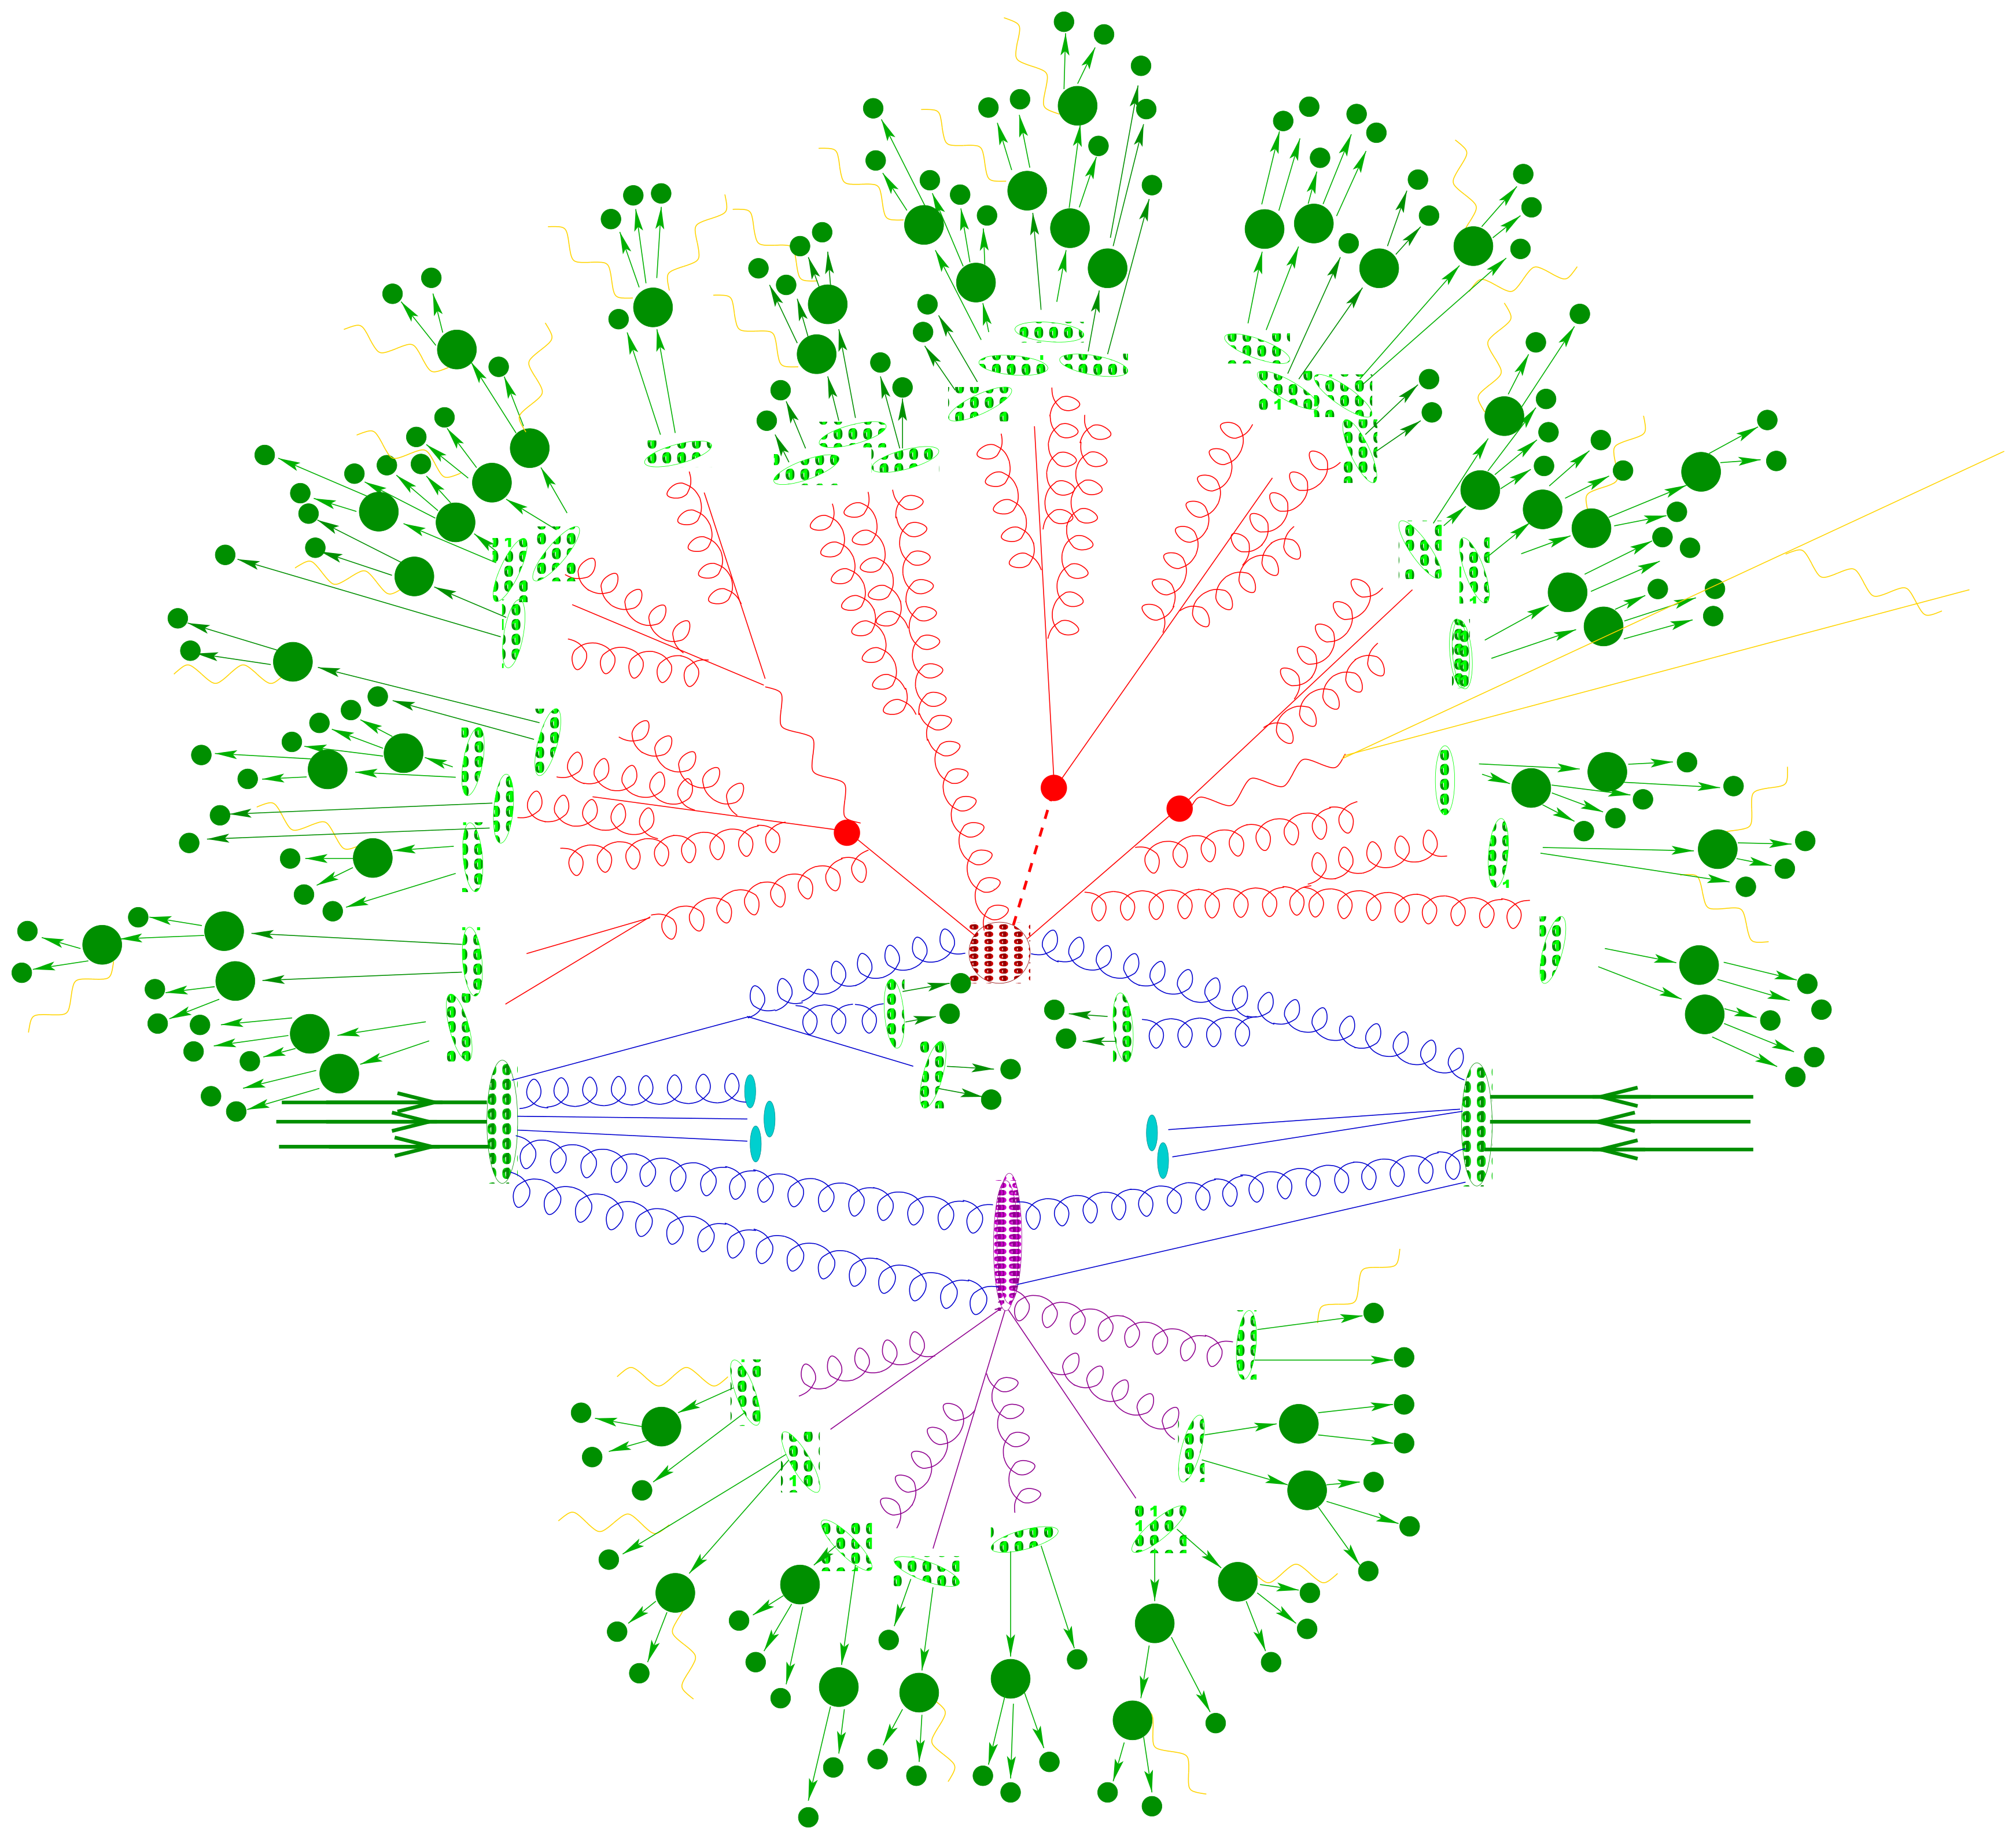
\includegraphics[width=0.9\textwidth]{parton_shower.png}
  \end{center}
\end{frame}


\begin{frame}{SM at the LHC}
\vspace{-.3cm}
\begin{columns}

\begin{column}{.50\textwidth}
\begin{block}{Top quark production}
\begin{itemize}\tiny
\item Heaviest quark in the SM 
\item LHC as a top machine $\to$ 6 tops/s (5 from pair, 1 from single)
\item 8 TeV: $\sigma_{t\bar{t}}=247.47\pm12.37$ pb, $\sigma_{t,\; \text{s-channel}}=5.56\pm0.22$ pb, $\sigma_{t,\; \text{t-channel}}=84.34\pm1.69$ pb and $\sigma_{tW}=22.2\pm0.67$ pb
\item $t\to bW^{-}$ with $Br(W^{+/-}\to l\nu)=0.33$ and $Br(W^{+/-}\to q\bar{q}')=0.67$
\item $m_{t}=173.34\pm 0.76$ \GeVcc
\end{itemize}
\end{block}

\vspace{-.4cm}
\begin{figure}[!Hhtbp]
  \begin{center}
    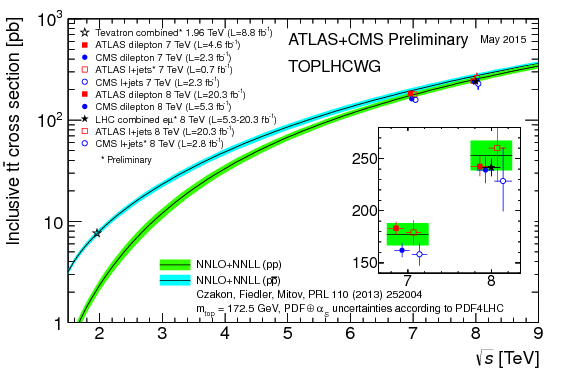
\includegraphics[width=1.0\textwidth]{../figs/toplhcwg_ttxsec_sqrts_may2015.png}
    %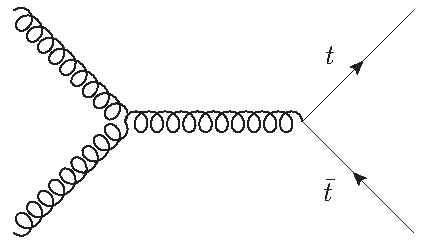
\includegraphics[width=0.3\textwidth]{../figs/Gluon_fusion_top_pair.jpg}
  \end{center}
\end{figure}
\end{column}

\begin{column}{.50\textwidth}
\begin{block}{Higgs boson production}
\begin{itemize}\tiny
\item Heaviest boson in the SM 
\item Rare process: 20 pb at 8TeV
\item Many decay channels: $Br(H^{o}\to b\bar{b})=0.57$
\item $m_{H}=125.09\pm 0.24$ \GeVcc~and $\sigma_{H}<20$ MeV
\end{itemize}
\end{block}

\vspace{-.2cm}
\begin{figure}[!Hhtbp]
  \begin{center}
    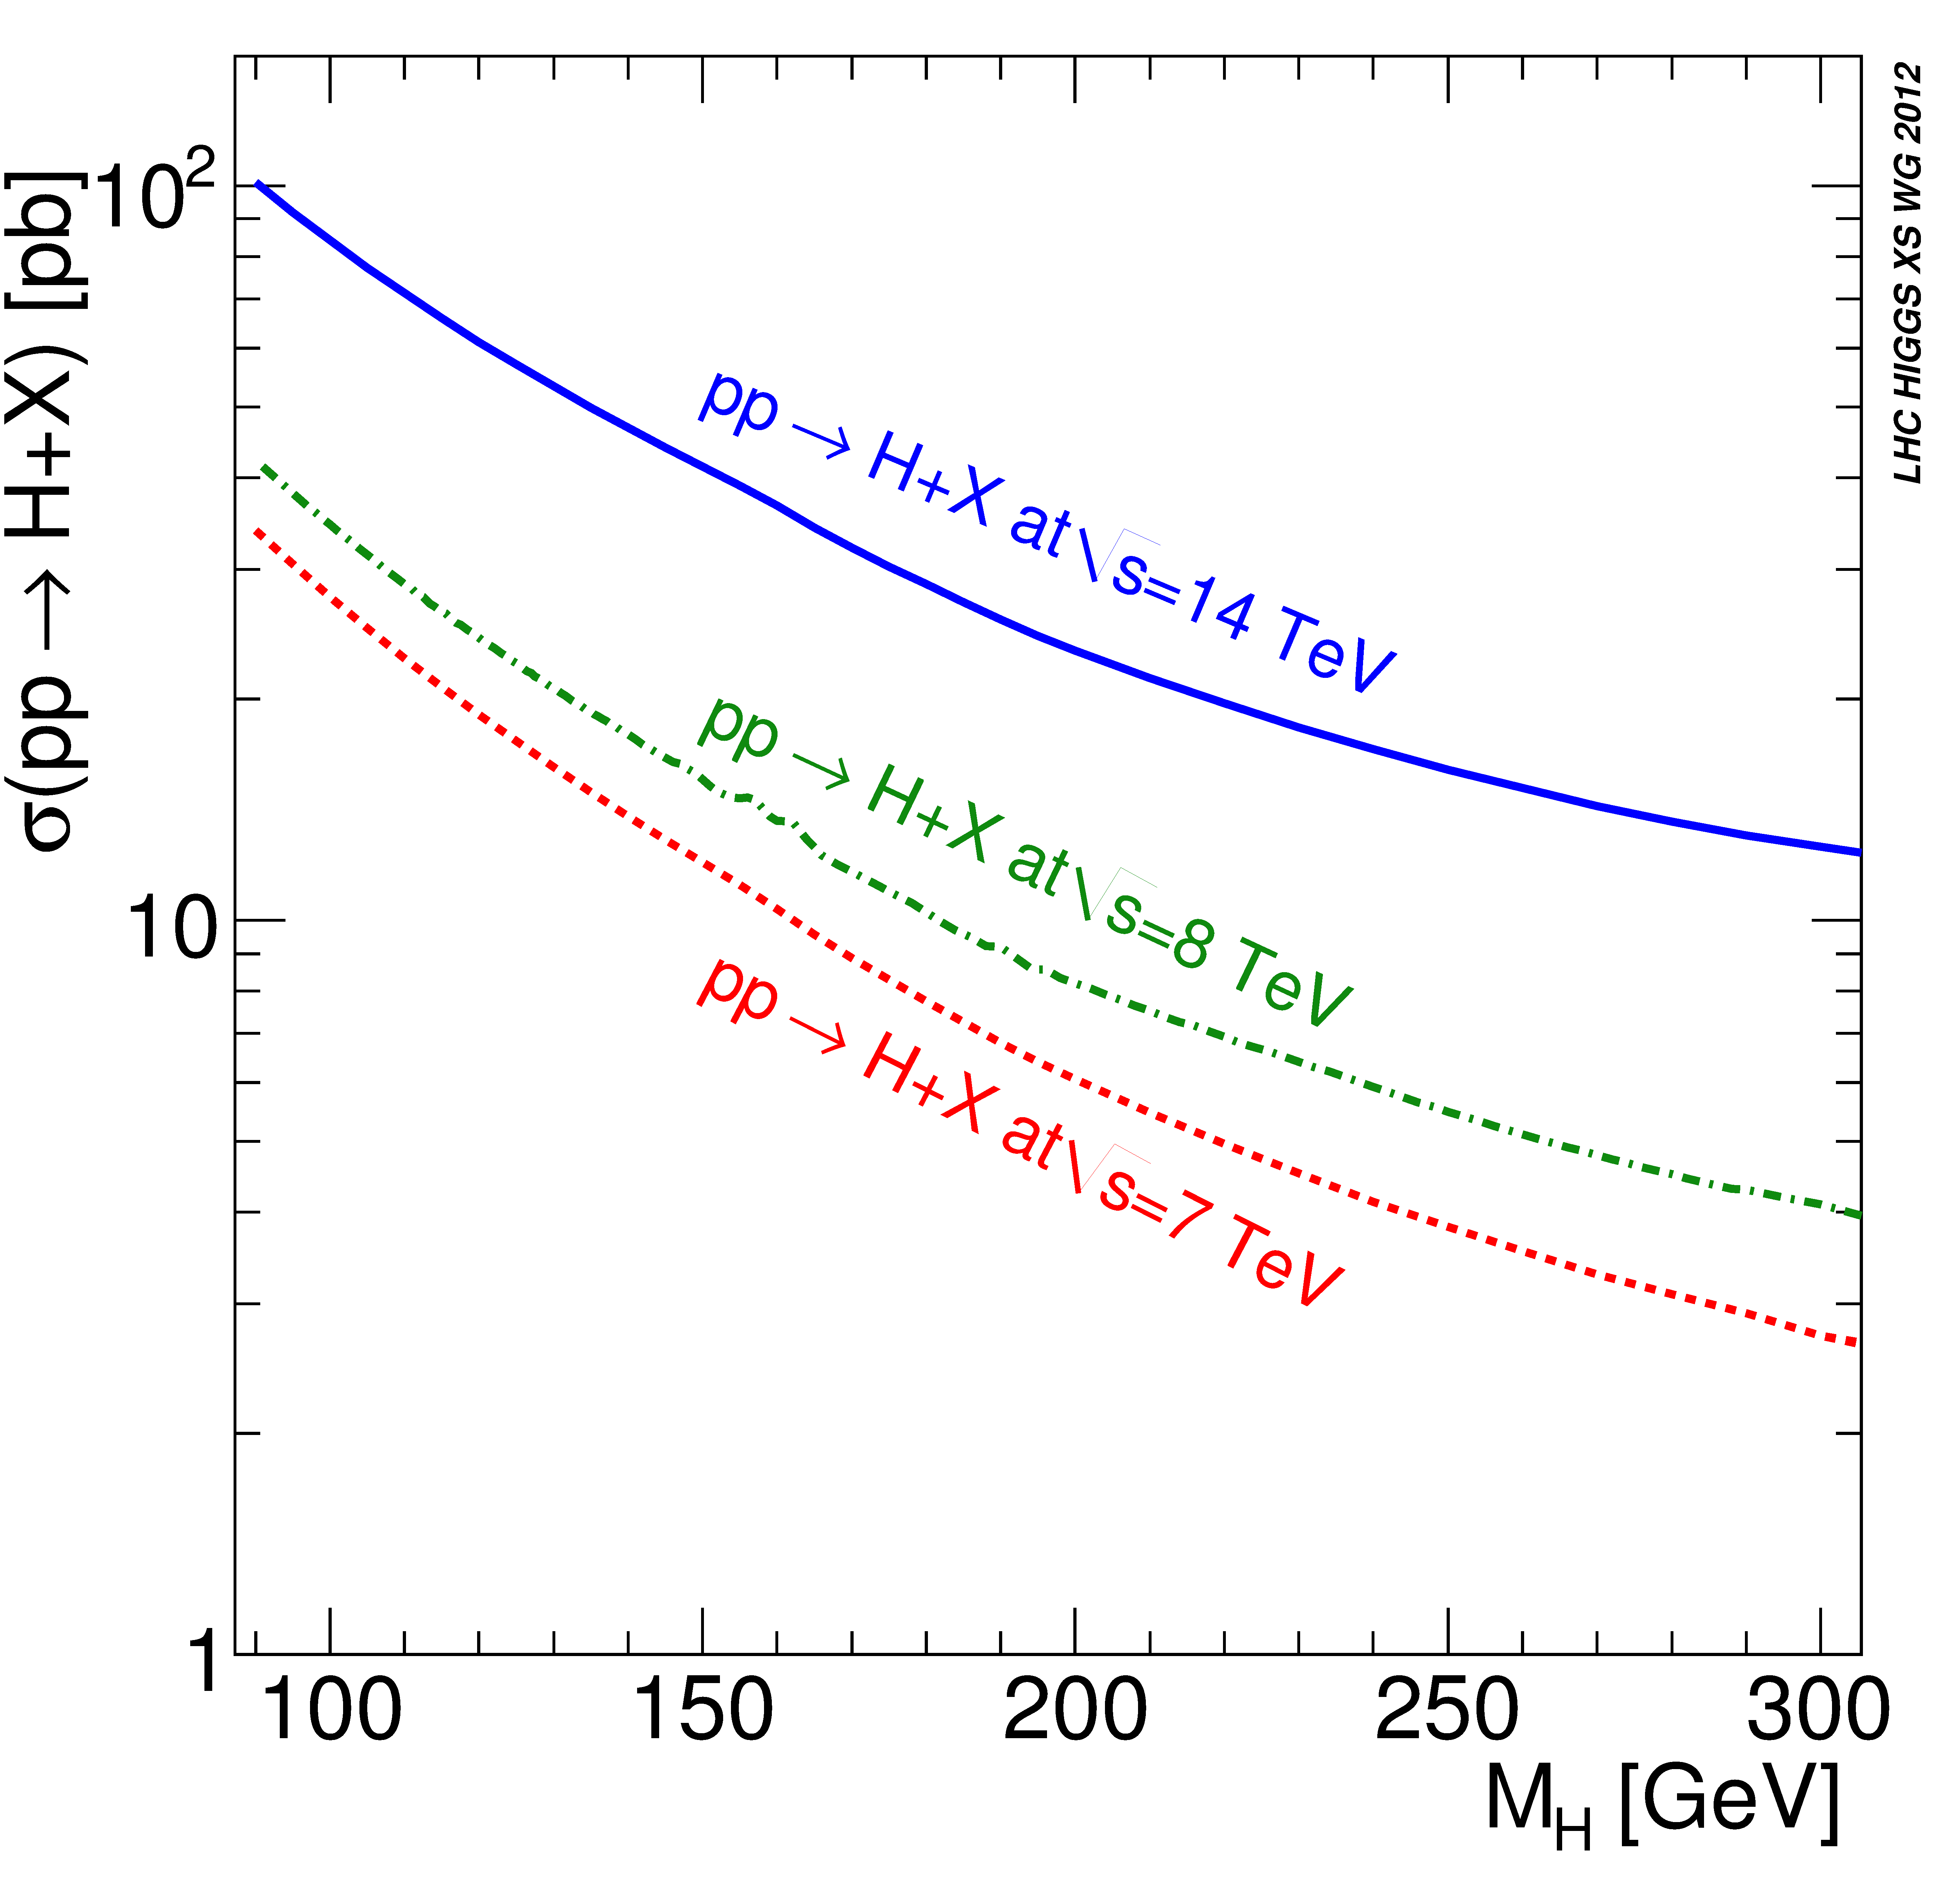
\includegraphics[width=0.8\textwidth]{../figs/totalXS_LM.png}
  \end{center}
\end{figure}

\end{column}
\end{columns}

\end{frame}

\fi

%%%%%%%%%%%%%%%%%%%%%%%%%%%%%%%%%%%%%%%%%%%%%%%%%%%%%%%%
%%%%%%%%%%%%%%%%%%%%%%%%%%%%%%%%%%%%%%%%%%%%%%%%%%%%%%%%
\section[CMS]{The CMS experiment at LHC}
\setcounter{tocdepth}{2}

\begin{frame}{}
The CMS experiment at LHC
\end{frame}

\subsection{CMS}

\begin{frame}{LHC}
\vspace{-.2cm}

\begin{columns}
\begin{column}{.50\textwidth}
\begin{figure}[!Hhtbp]
  \begin{center}
    \includegraphics[width=1.0\textwidth]{lhc_underground.jpg}
  \end{center}
\end{figure}
\vspace{-.2cm}
\begin{block}{}
\begin{itemize}\scriptsize
\item Proton and heavy ion collider
\item 27 km of circumference, 100 m underground
\item 1232 superconductor magnets at 1.9 K with a magnetic field of 8.33 T
\item Run 1: 4 TeV/proton
\item Run 2: 6.5 TeV/proton, started last June
\end{itemize}
\end{block}
\end{column}

\begin{column}{.50\textwidth}
\begin{block}{}
\begin{itemize}\scriptsize
\item In run 1: Around 1000 proton bunches, spaced 50 ns $\to$ 20 millions of collisions / s
\item Main experiments:
  \begin{itemize}\tiny
  \item Generic purpose: ATLAS and CMS
  \item Beauty physics: LHCb
  \item Quark-Gluon plasma: ALICE
  \item Forward physics: LHCf, TOTEM
  \end{itemize}
\end{itemize}
\end{block}
\vspace{-.2cm}
\begin{figure}[!Hhtbp]
  \begin{center}
    \includegraphics[width=1.0\textwidth]{lhc_hall_1.jpg}
  \end{center}
\end{figure}
\end{column}
\end{columns}

\end{frame}


\begin{frame}{}
\vspace{-.2cm}

\begin{columns}
\begin{column}{.50\textwidth}
\begin{figure}[!Hhtbp]
  \begin{center}
    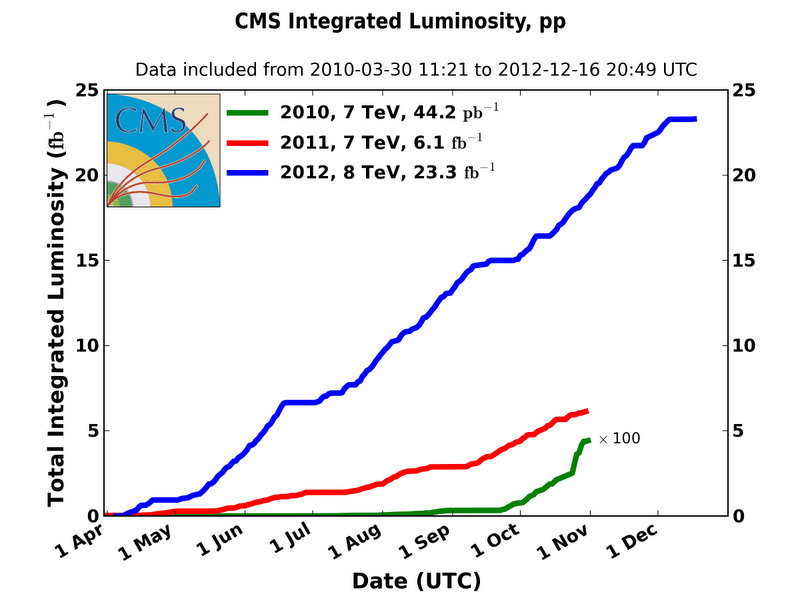
\includegraphics[width=1.0\textwidth]{../figs/cms-int-10to12.jpg}
    %\caption{CMS integrated luminosity for proton-proton collisions delivered by LHC. }
    %\label{fig:CMSlumi}
  \end{center}
\end{figure}
\vspace{-.5cm}
\begin{figure}[!Hhtbp]
  \begin{center}
    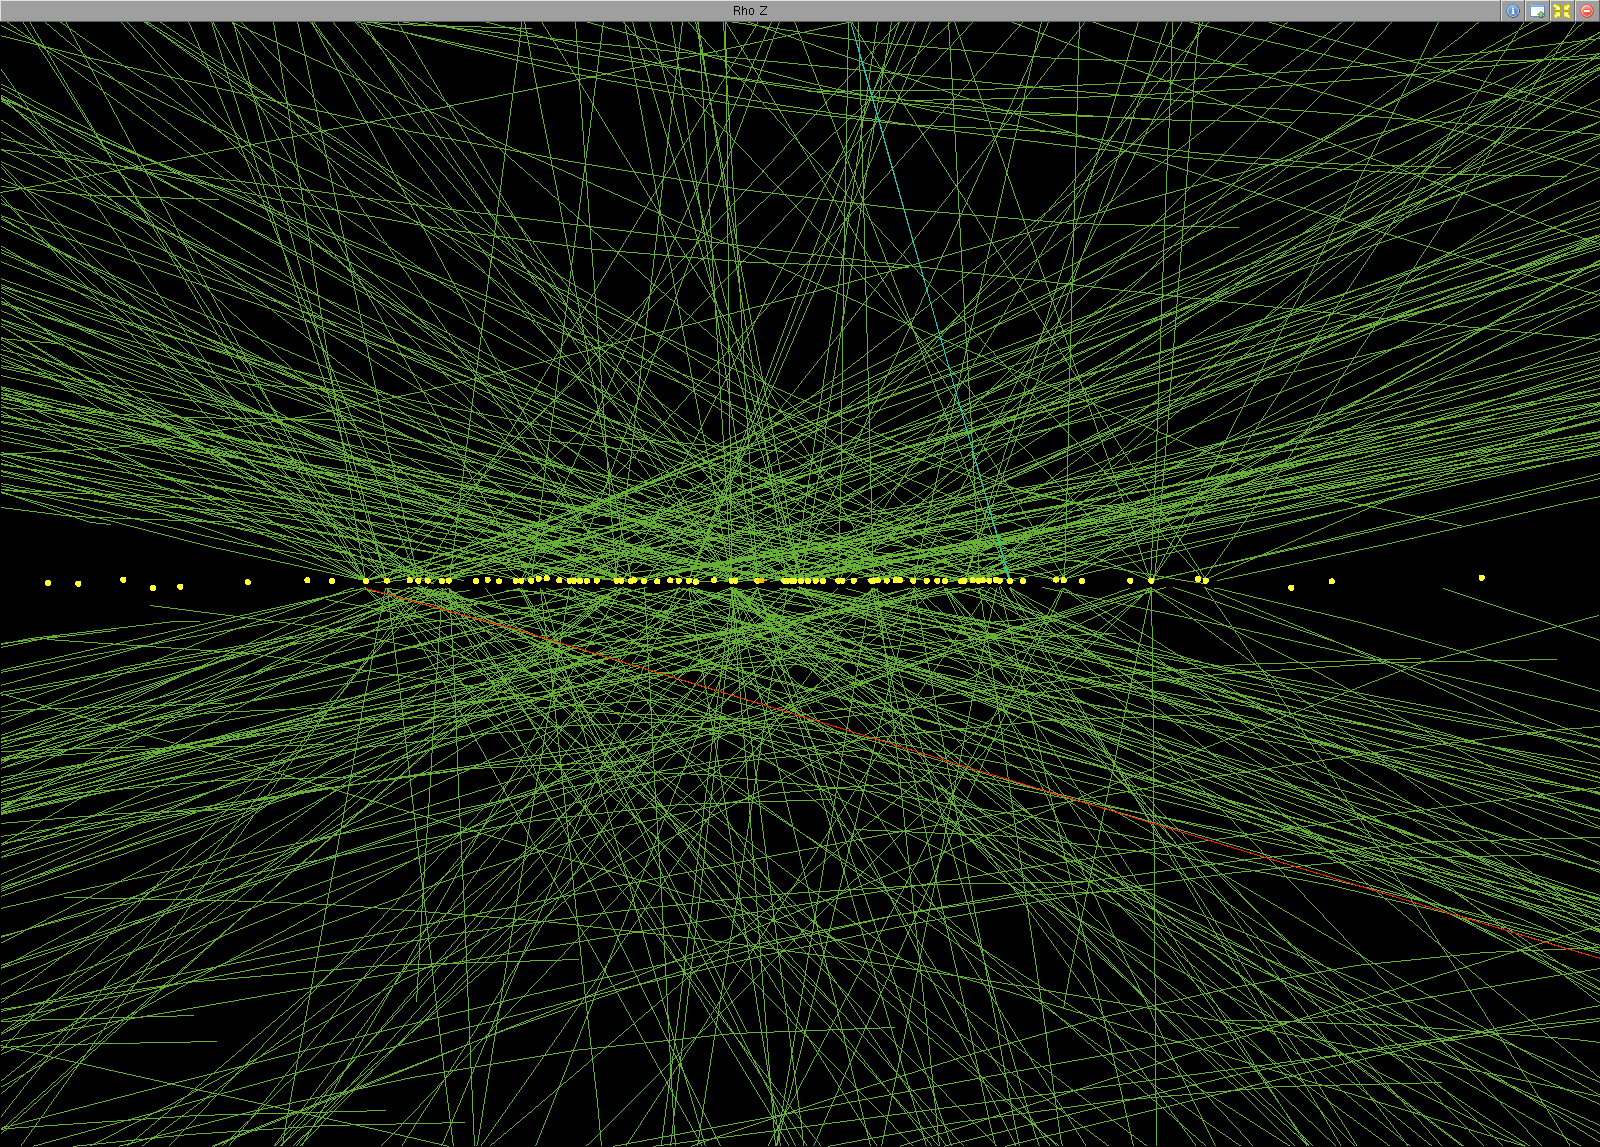
\includegraphics[width=1.0\textwidth]{../figs/pileup.png}
    %\caption{High pile-up event (78 interactions) seen by CMS detector. Event 35655522, from 198609 run, lumi 56, recorded on 2012.}% Image credit: Andre Holzner }                                        
    %\label{fig:pileup}
  \end{center}
\end{figure}
\end{column}

\begin{column}{.50\textwidth}
\begin{block}{}
\begin{equation*}
  L=\frac{k_{b}N_{b}^{2}f_{rev}}{4\pi\sigma^{*}_{x}\sigma^{*}_{y}}R                                     
\end{equation*}
\begin{equation*}
  N_{events}=L\times \sigma_{process} \times \epsilon
\end{equation*}
\end{block}

\tiny{
%\begin{table}[htbH]
\begin{center}
%\resizebox{\textwidth}{!}{
\begin{tabular}{|c|c c|}
\hline
 & 2012 & Nominal \\
\hline
Energy [GeV]& 4000 & 7000 \\
Inst. Lumi. [$\text{cm}^{-2}\text{s}^{-1}$] & 7.54$\times10^{33}$ & $10^{34}$ \\
$k_{b}$ Number of bunches & 1374 & 2808 \\
Bunch spacing [ns] & 50 & 25 \\
\hline
\end{tabular}
%}
\end{center}
%\end{table}
}%

\begin{block}{}
\begin{itemize}\scriptsize
\item Increasing the recorded luminosity, increases the sensitivity to rare processes.
\item Run 1: 19.7 fb$^{-1}$ in 2012 \MVAt~8 TeV
\end{itemize}
\end{block}
\begin{block}{}
\scriptsize PileUp: 20 interactions per crossing during 2012
\end{block}
\end{column}
\end{columns}

\end{frame}

\begin{frame}{CMS: Compact Muon Solenoid}
\vspace{-.2cm}

\begin{figure}[!Hhtbp]
  \begin{center}
    \includegraphics[width=\textwidth]{cms_det.png}
  \end{center}
\end{figure}

\end{frame}


\begin{frame}{Sub-detectors}
\vspace{-.2cm}
\begin{figure}[!Hhtbp]
  \begin{center}
    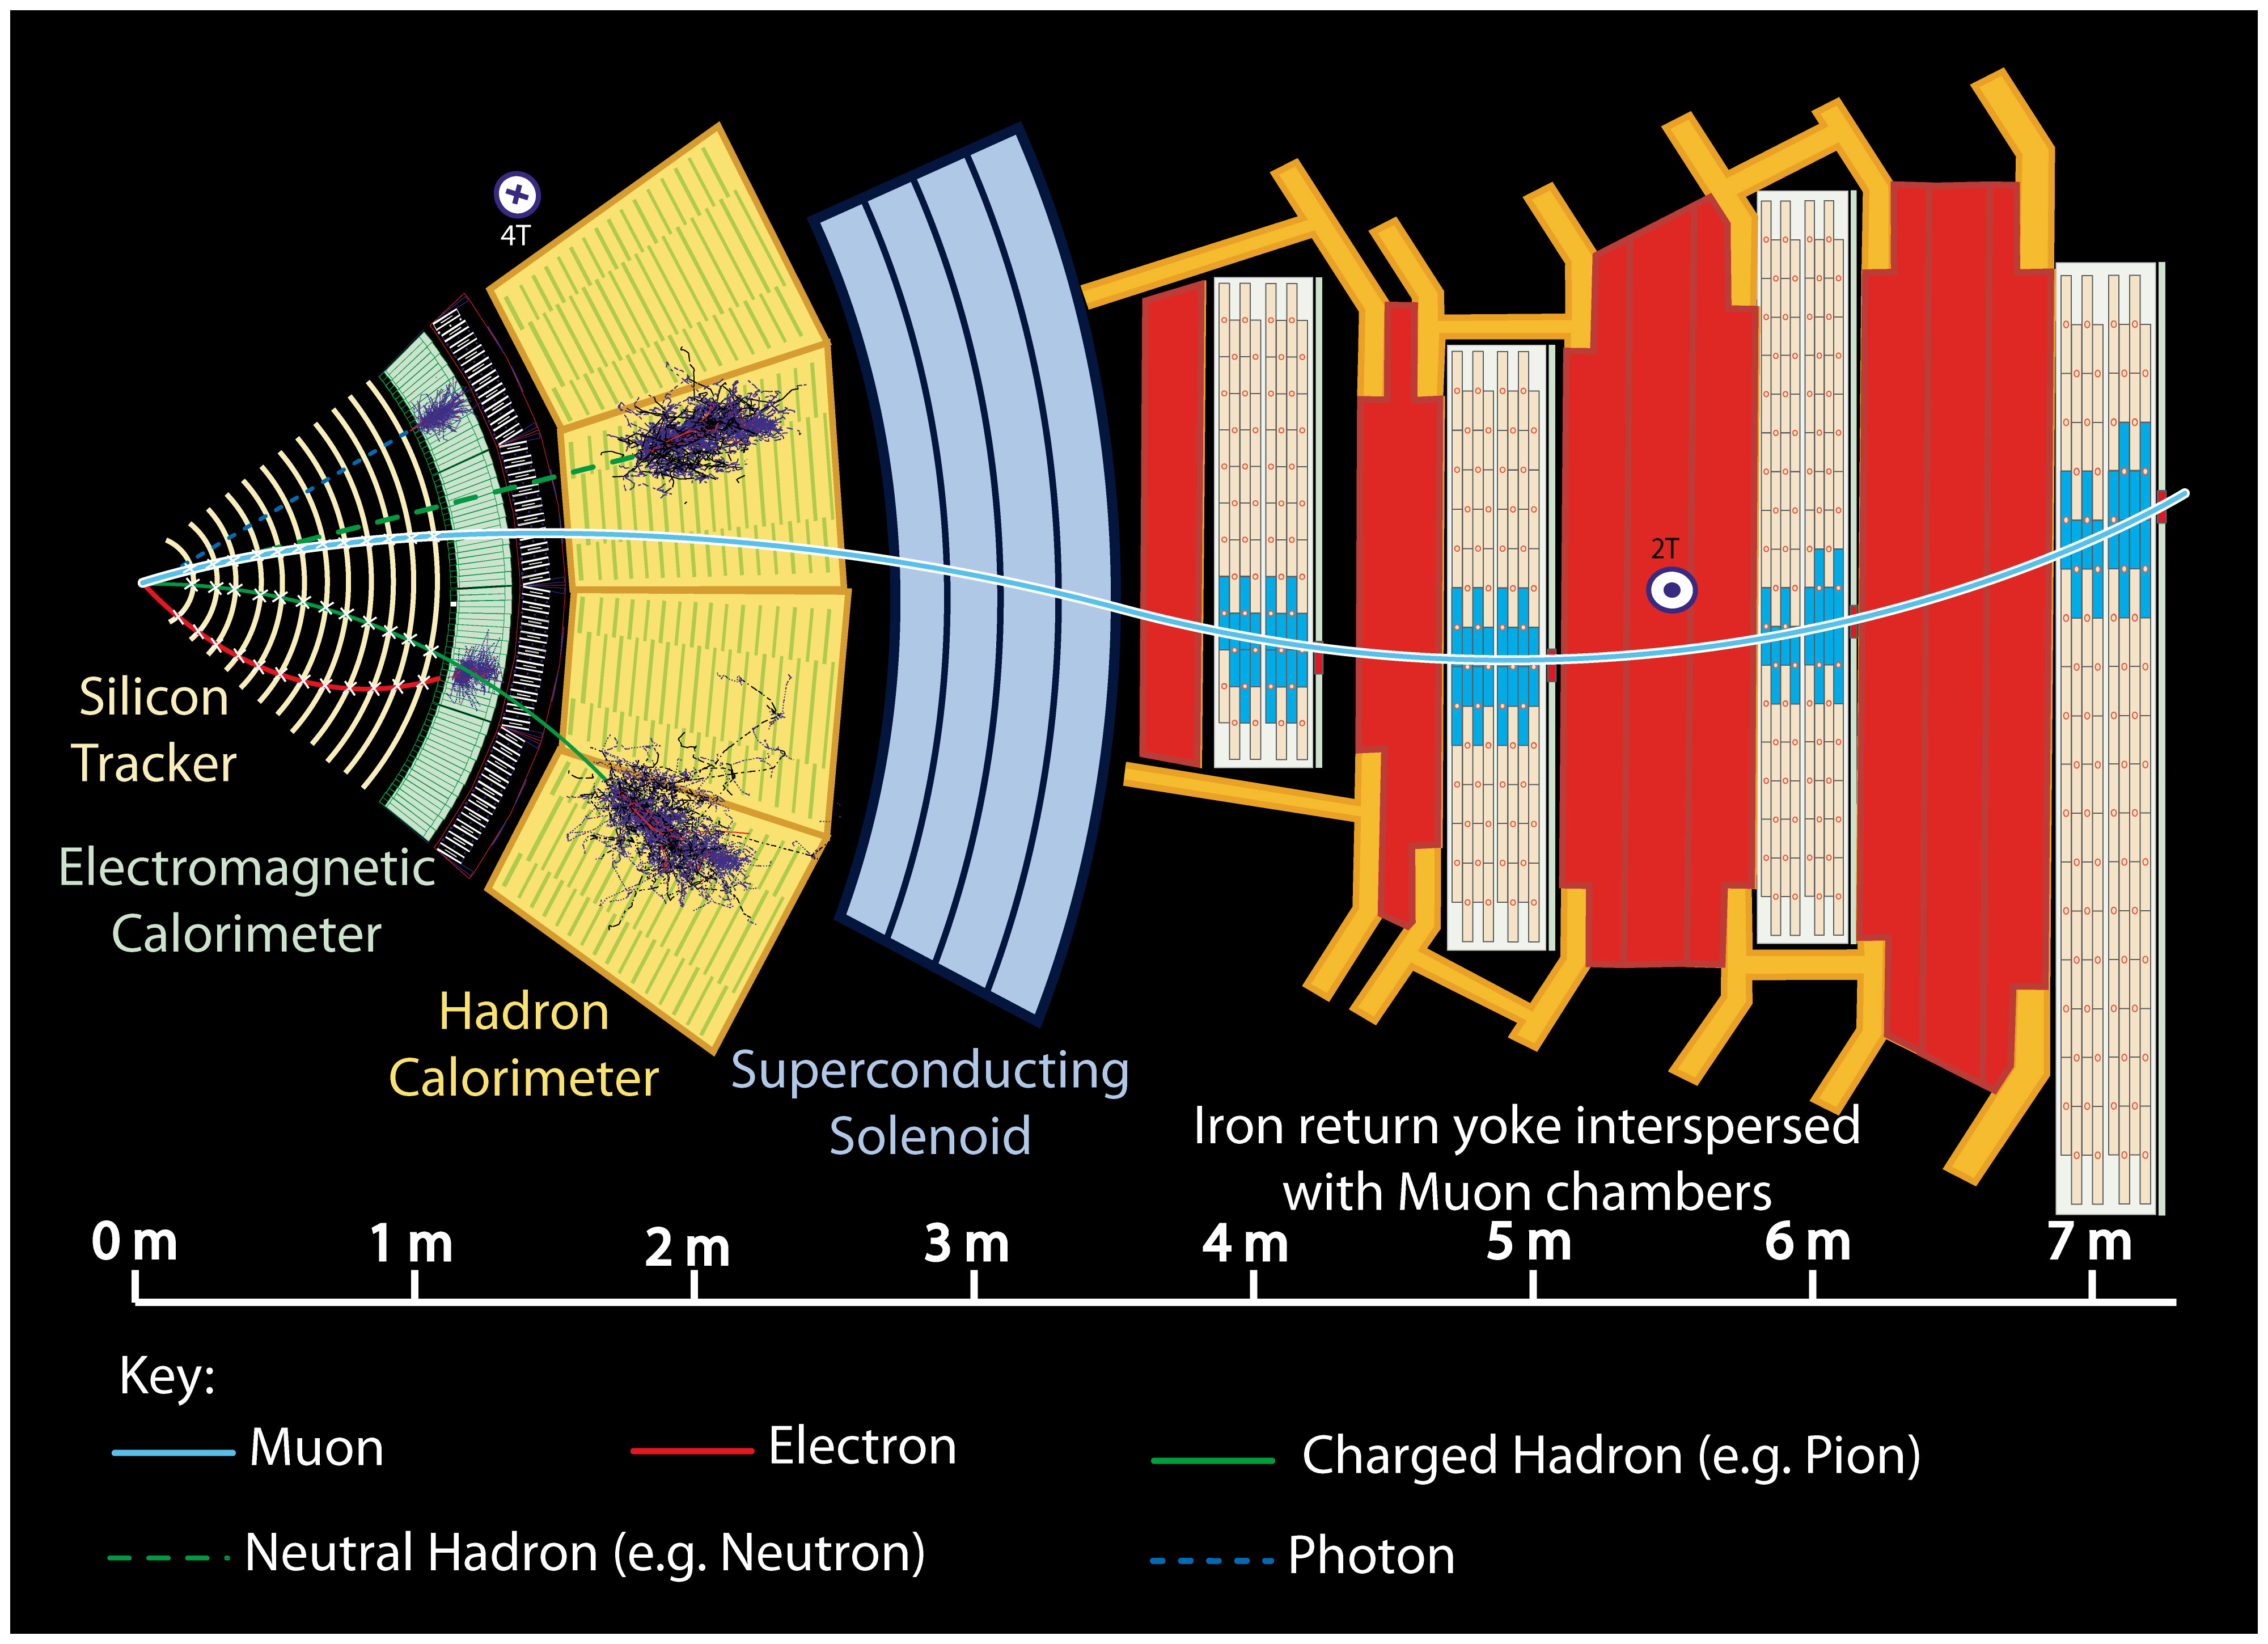
\includegraphics[width=0.7\textwidth]{../figs/PictureforPoint5_oct04_allp.jpg}
    %\caption{CMS sub-detectors and particle identification. }
    %\label{fig:cmsslice}
  \end{center}
\end{figure}
\vspace{-.4cm}
\begin{block}{}
\begin{itemize}\tiny
\item Tracker system: Pixel system (vertex reconstruction) and Silicon strips (Measurement of \pt~of charged particles)
\item Electromagnetic calorimeter (ECAL): 80000 crystals for the measurement of electrons and photons energy
\item Hadron calorimeter (HCAL): Absorber and scintillator to measure the energy of hadrons
\item Muon chambers: RPC, DT and CSC to measure muons \pt
\end{itemize}
\end{block}

\end{frame}


\begin{frame}{}
\vspace{-.2cm}

%\begin{center}
\begin{textblock}{95}(0,6)
    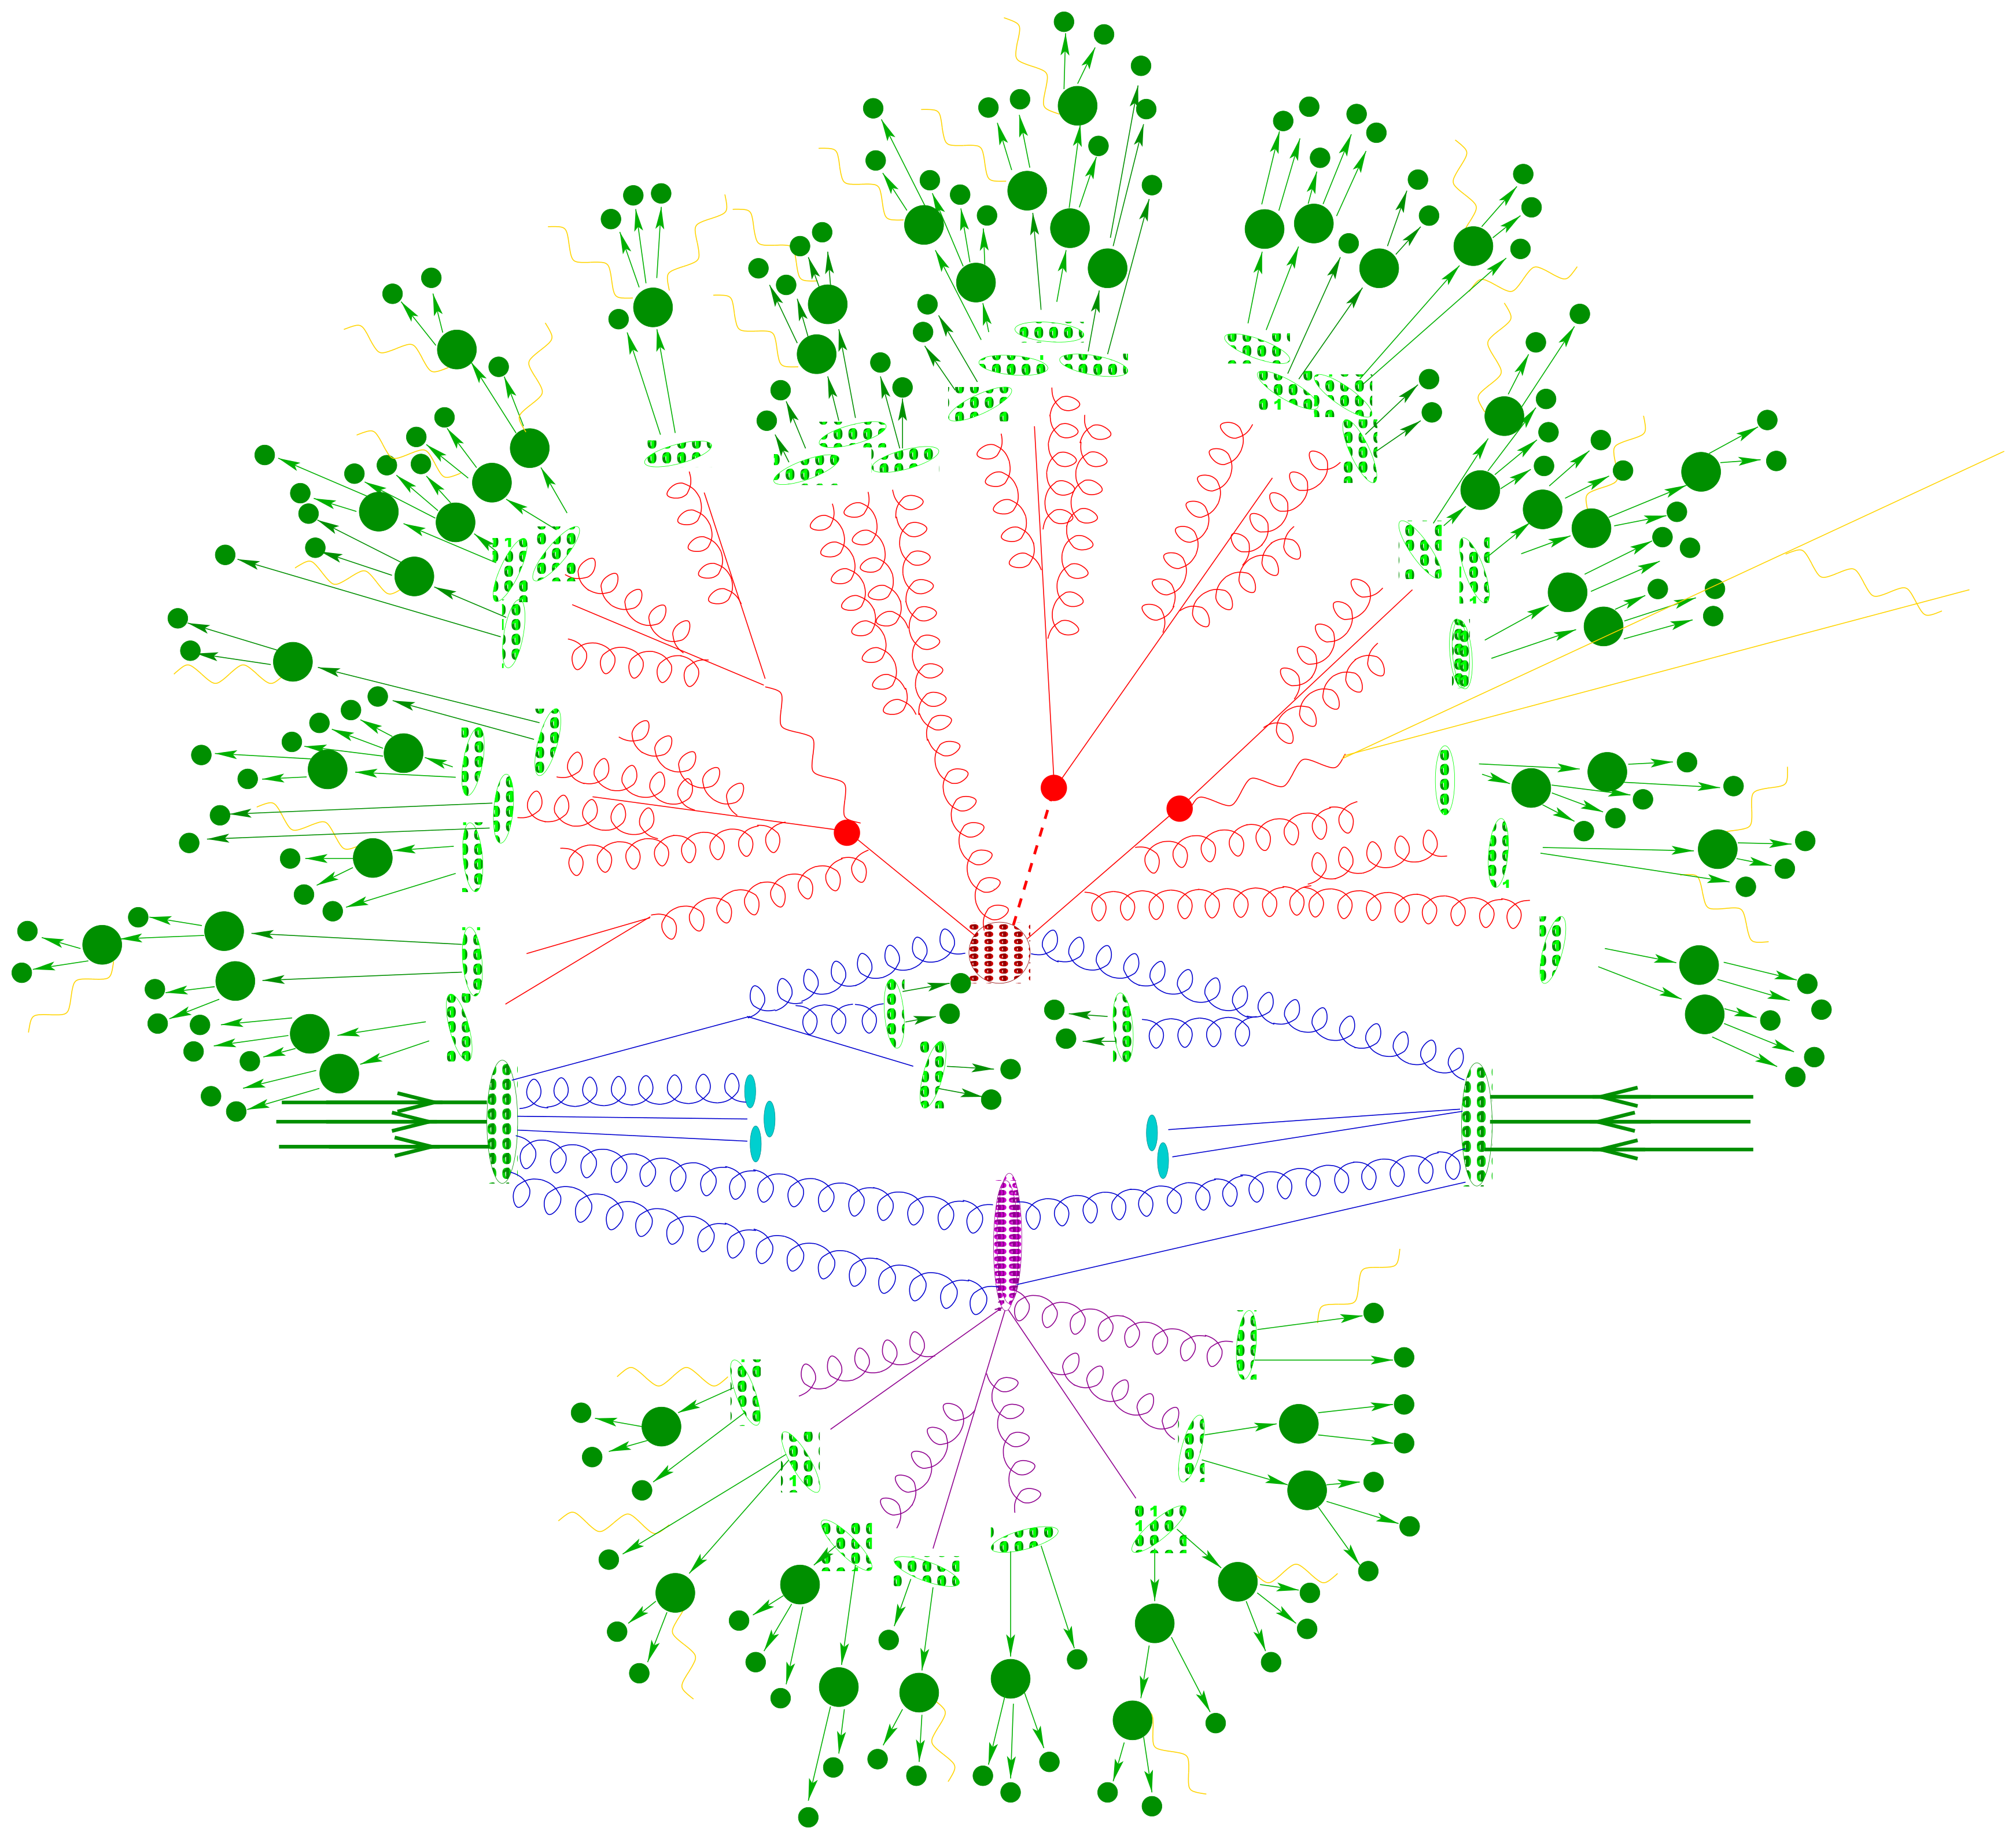
\includegraphics[width=1.0\textwidth]{parton_shower.png}
\end{textblock}
%  \end{center}
\end{frame}



\begin{frame}{Monte-Carlo simulation}
\vspace{-.4cm}
\begin{columns}
\begin{column}{.50\textwidth}
  \begin{block}{MadGraph}\tiny
    Simulation of hard interaction in collisions \\
    \textbf{Figure}: \Z+jets production, \Z~$\to$ neutrinos \MVAt~8 TeV
  \end{block}
\vspace{-.5cm}
\begin{figure}[!Hhtbp]
  \begin{center}
    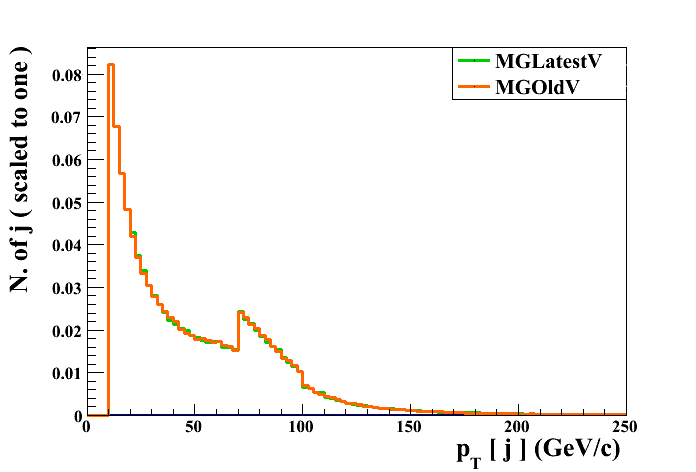
\includegraphics[width=0.9\textwidth]{ZjetsRelVal1.png}\\
    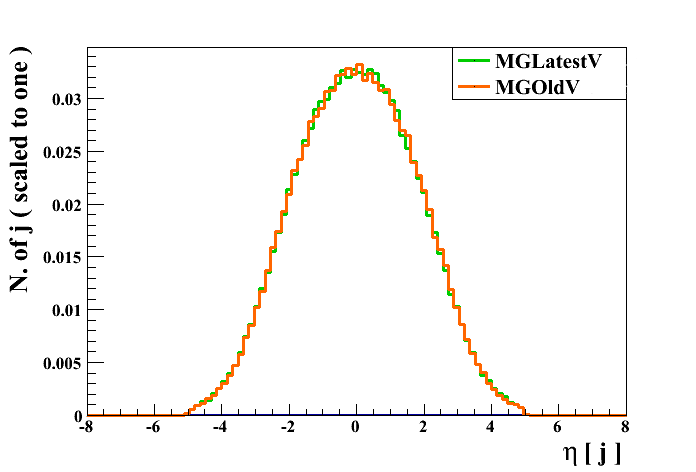
\includegraphics[width=0.9\textwidth]{ZjetsRelVal2.png}
  \end{center}
\end{figure}
\end{column}

\begin{column}{.50\textwidth}
  \begin{block}{RIVET toolkit}\tiny
    \textbf{Pythia}: Simulation of hadronization and showering \\
    Comparison of different generators with real data %\\
    %\textbf{Figure}: \W~boson $p_{T}$ measured by ATLAS experiment in muon final states compared to different MC simulations. py6 stands for Pythia 6, py8 for Pythia 8, MGpy6 MadGraph interfaced with Pythia 6 and PWG for Powheg. MadGraph with Pythia 6 gives the best description of experimental data.
  \end{block}
  \begin{figure}[!Hhtbp]
  \begin{center}
    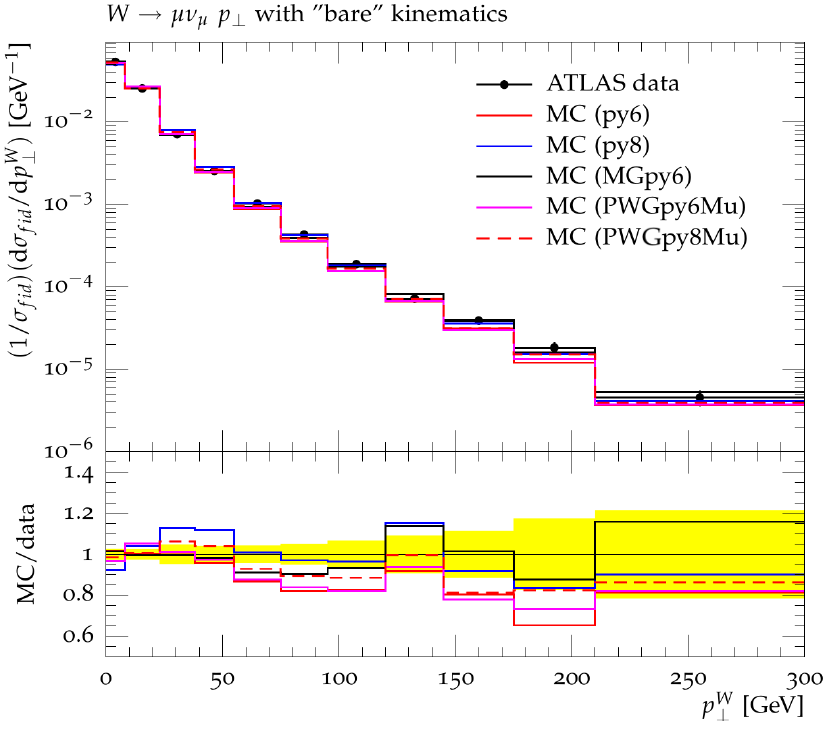
\includegraphics[width=1.0\textwidth]{Wpt_rivet.png}
  \end{center}
\end{figure}
\end{column}
\end{columns}

\end{frame}



\begin{frame}{Interface between partonic and hadronic simulation}
\vspace{-.2cm}
\begin{columns}
\begin{column}{.50\textwidth}
  \begin{block}{}\tiny
    Possible overlap between parton shower and matrix element when adding extra jets. MLM merging:
    \begin{itemize}
    \item $N^{ME}(j)$ \MVAt~parton level
    \item $N^{PS}(j)$ after parton shower
    \item Compare $N^{ME}(j)$ and $N^{PS}(j)$
    \end{itemize}
  \end{block}
\end{column}
\begin{column}{.50\textwidth}
  \begin{block}{}\tiny
    To study the correctness of the choice:
    \begin{itemize}
    \item DJR diagrams
    \item Transition between $n$ and $n-1$ jet multiplicities as a function of the merging scale
    \end{itemize}
  \end{block}
\end{column}
\end{columns}

\vspace{-.2cm}
\begin{columns}
\begin{column}{.30\textwidth}
\begin{figure}[!Hhtbp]
  \begin{center}
    \includegraphics[width=1.3\textwidth]{ExplainDJR.png}
  \end{center}
\end{figure}
\end{column}
\begin{column}{.70\textwidth}
\begin{figure}[!Hhtbp]
  \begin{center}
    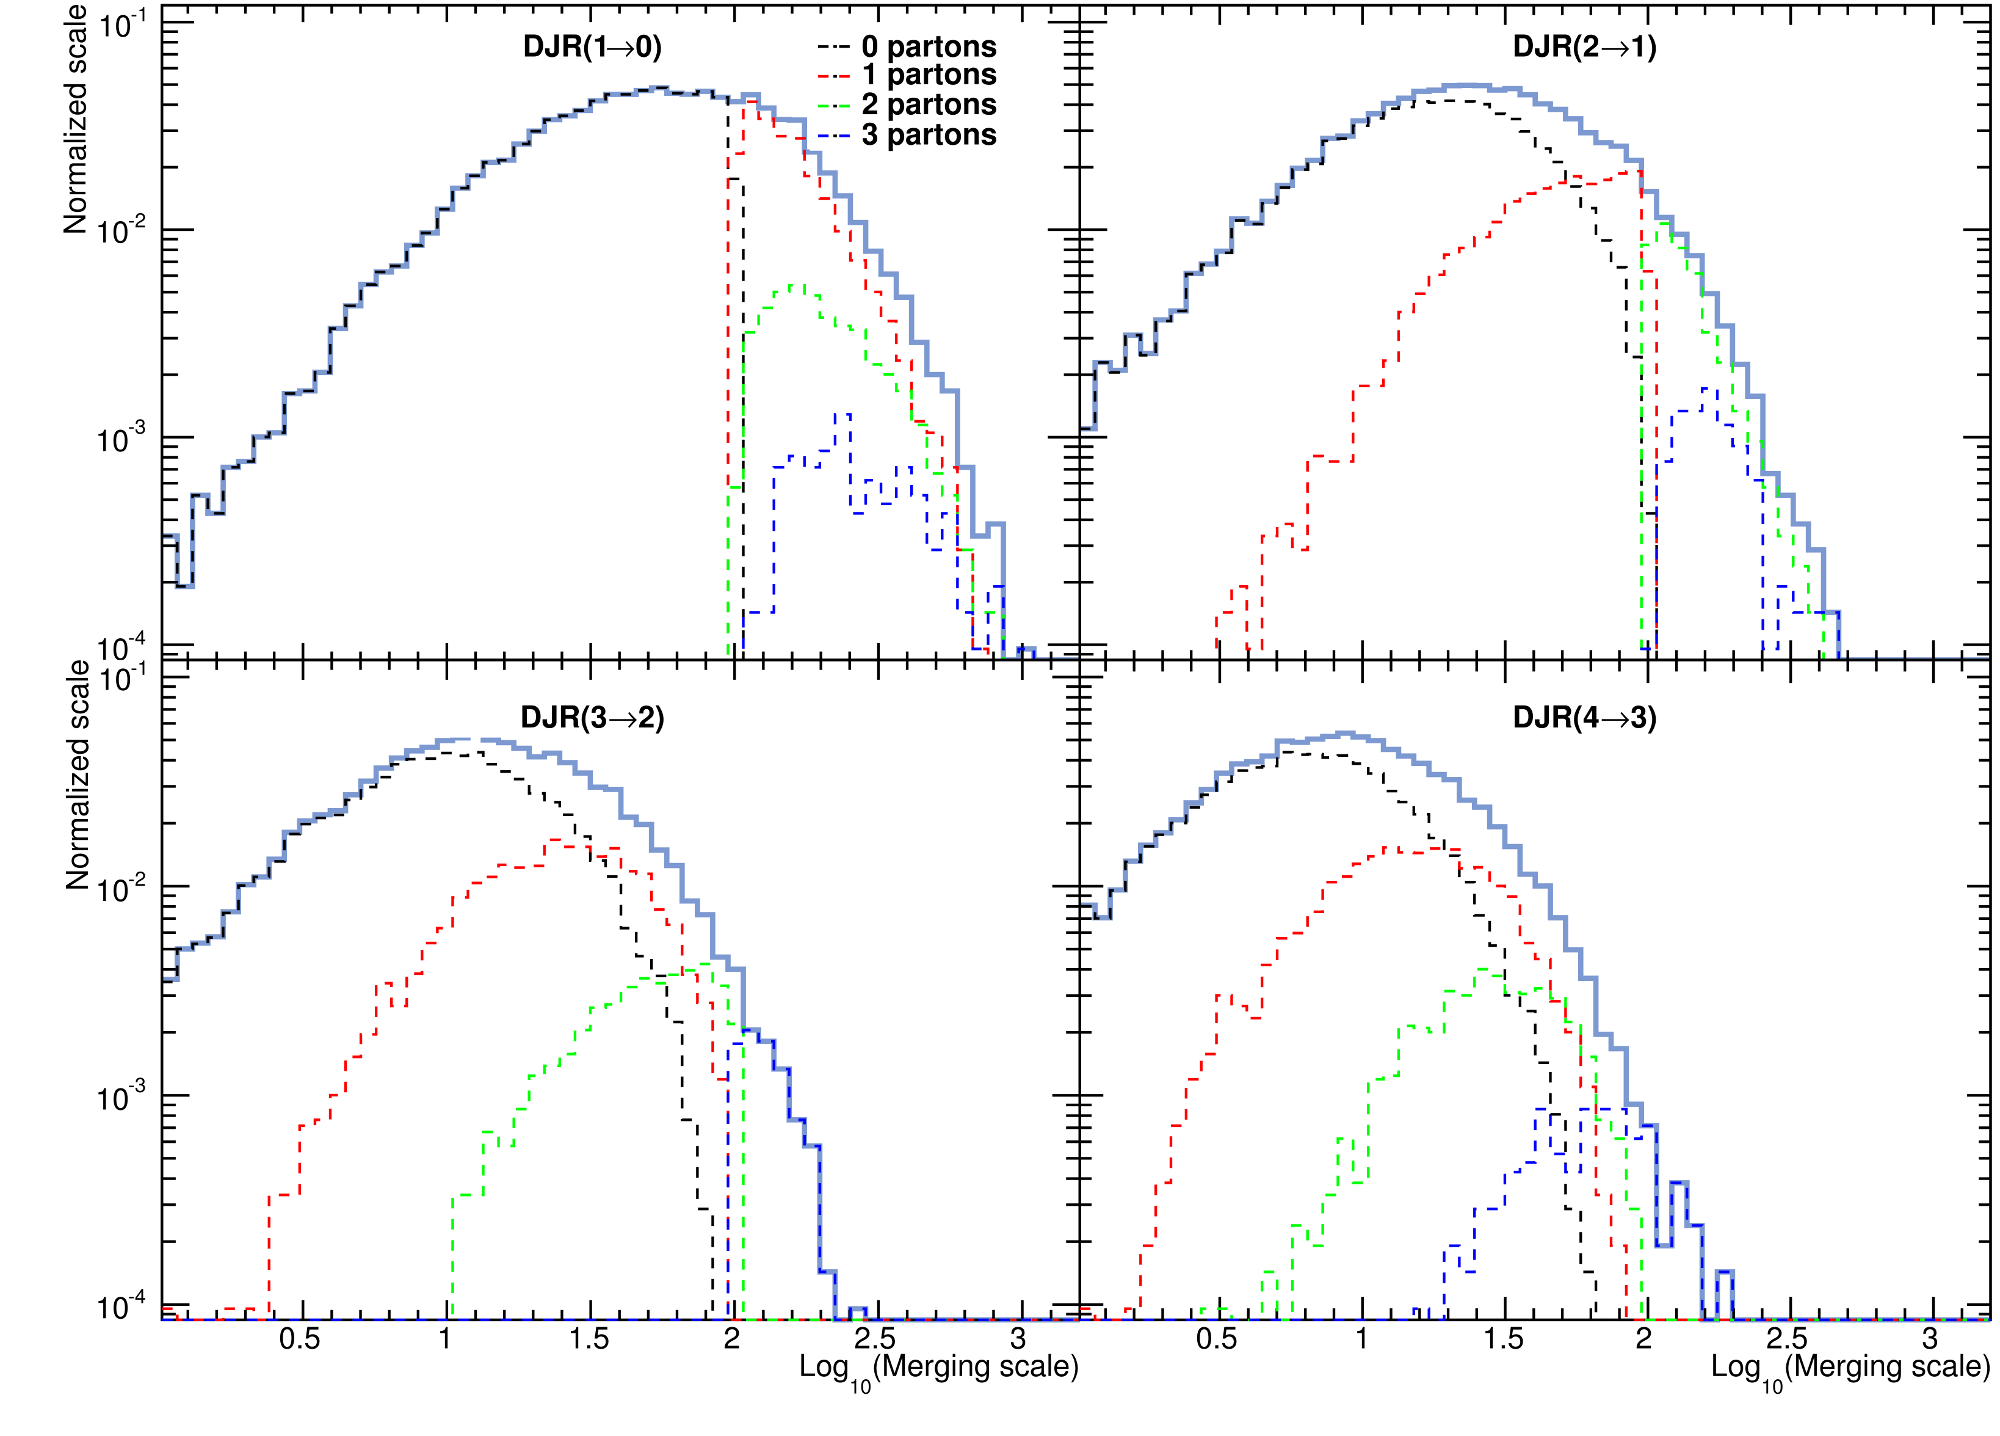
\includegraphics[width=1.0\textwidth]{../figs/DJR_q100_xq20_TTJets13TeV.png}
  \end{center}
\end{figure}
\end{column}
\end{columns}


%\begin{figure}[!Hhtbp]
%  \begin{center}
%    \includegraphics[width=0.3\textwidth]{ExplainDJR.png}
%    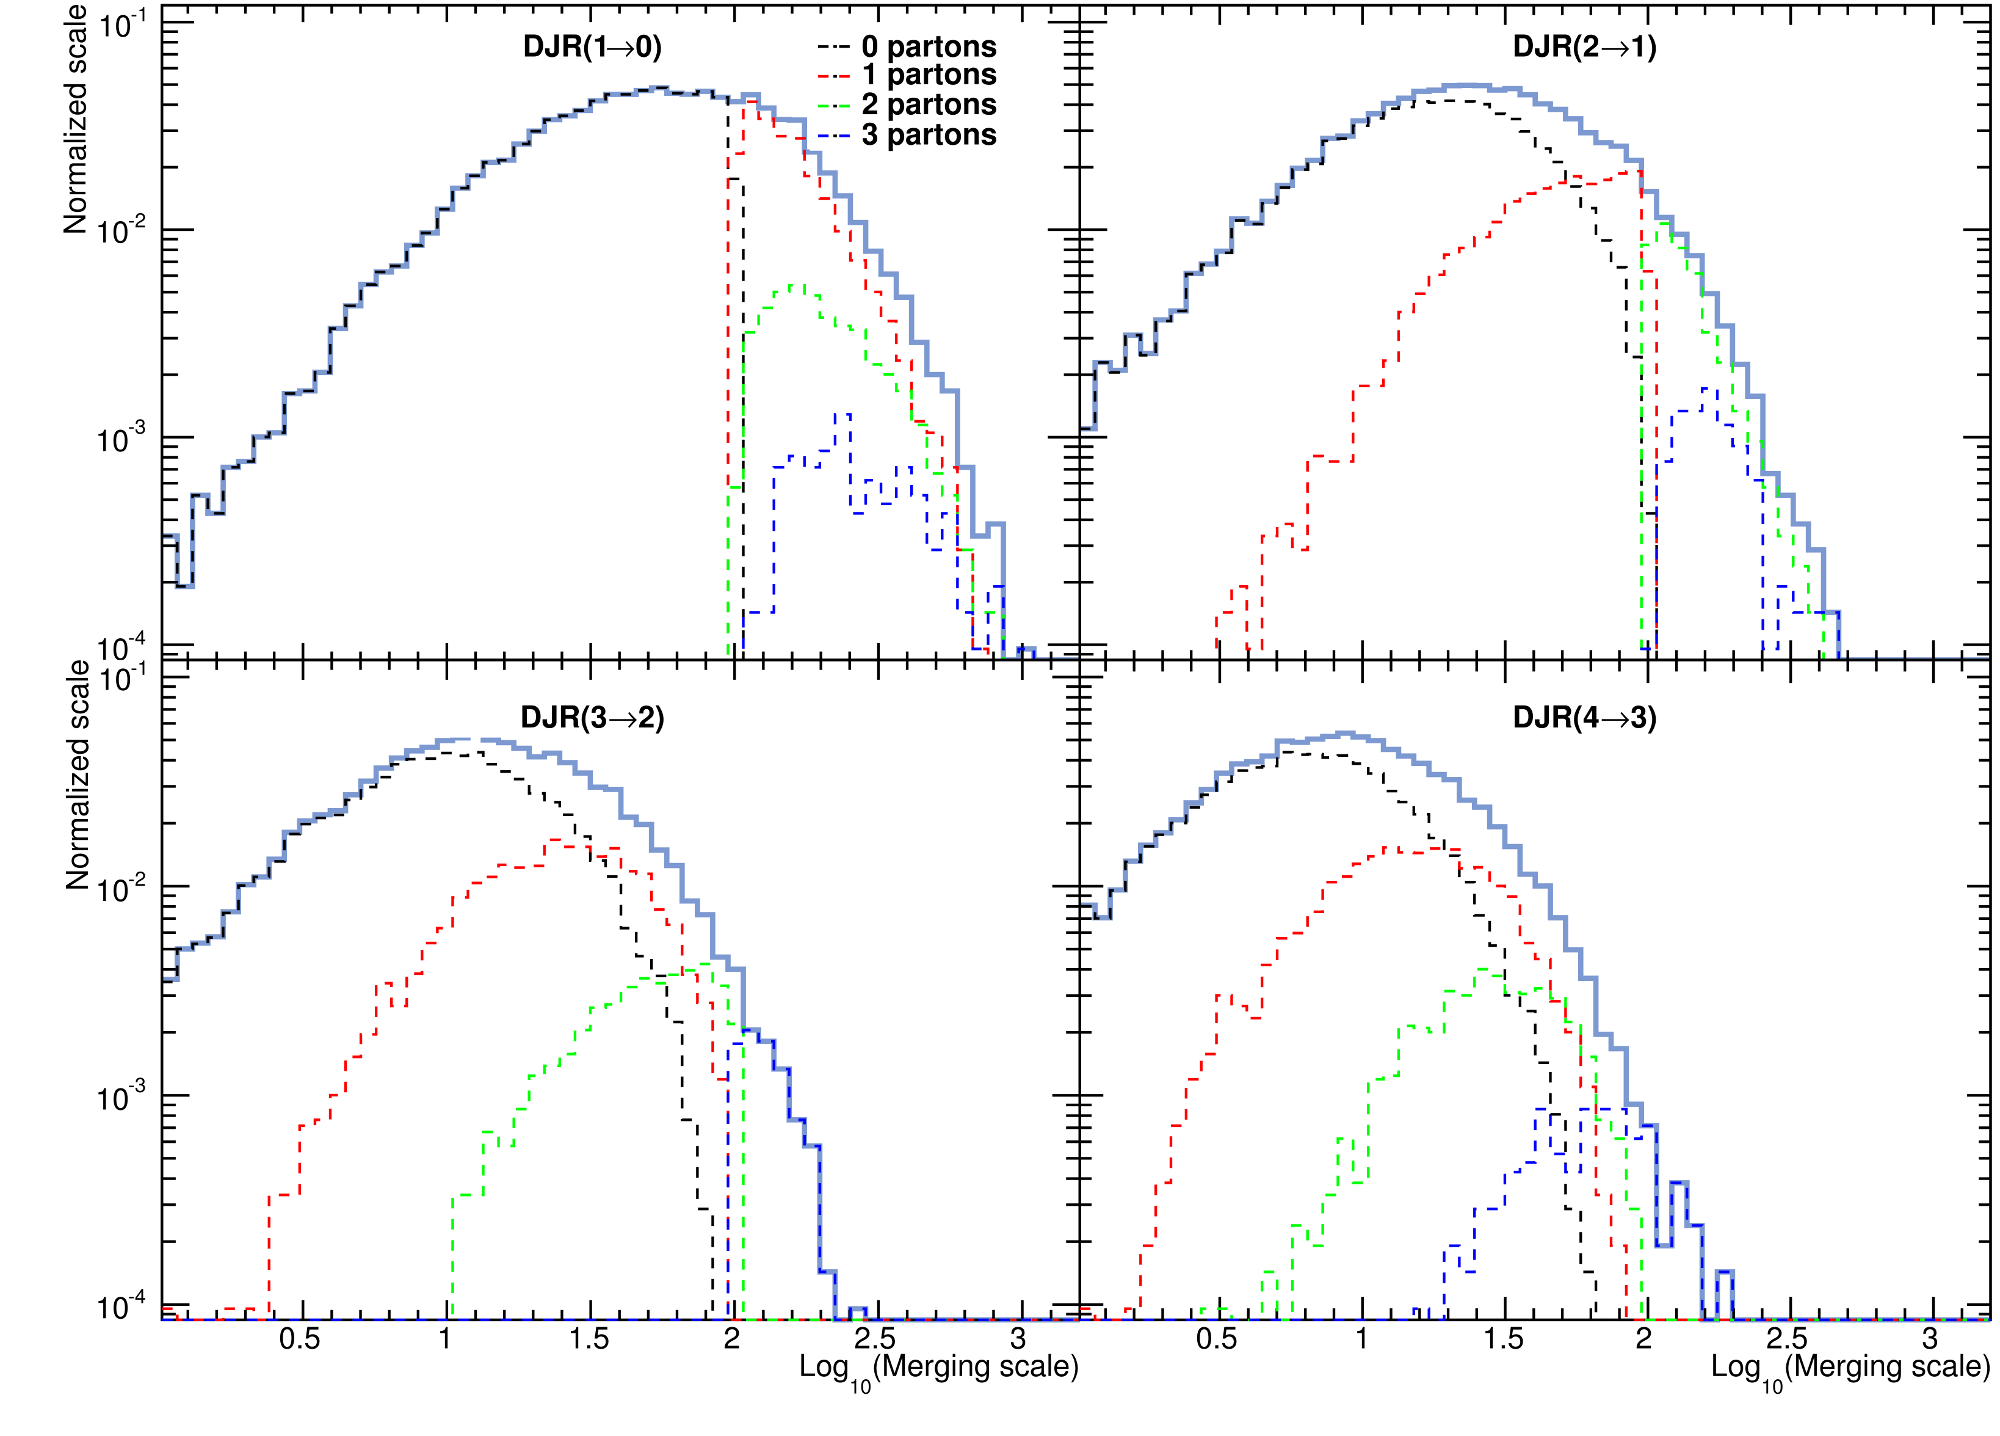
\includegraphics[width=0.7\textwidth]{../figs/DJR_q100_xq20_TTJets13TeV.png}
    %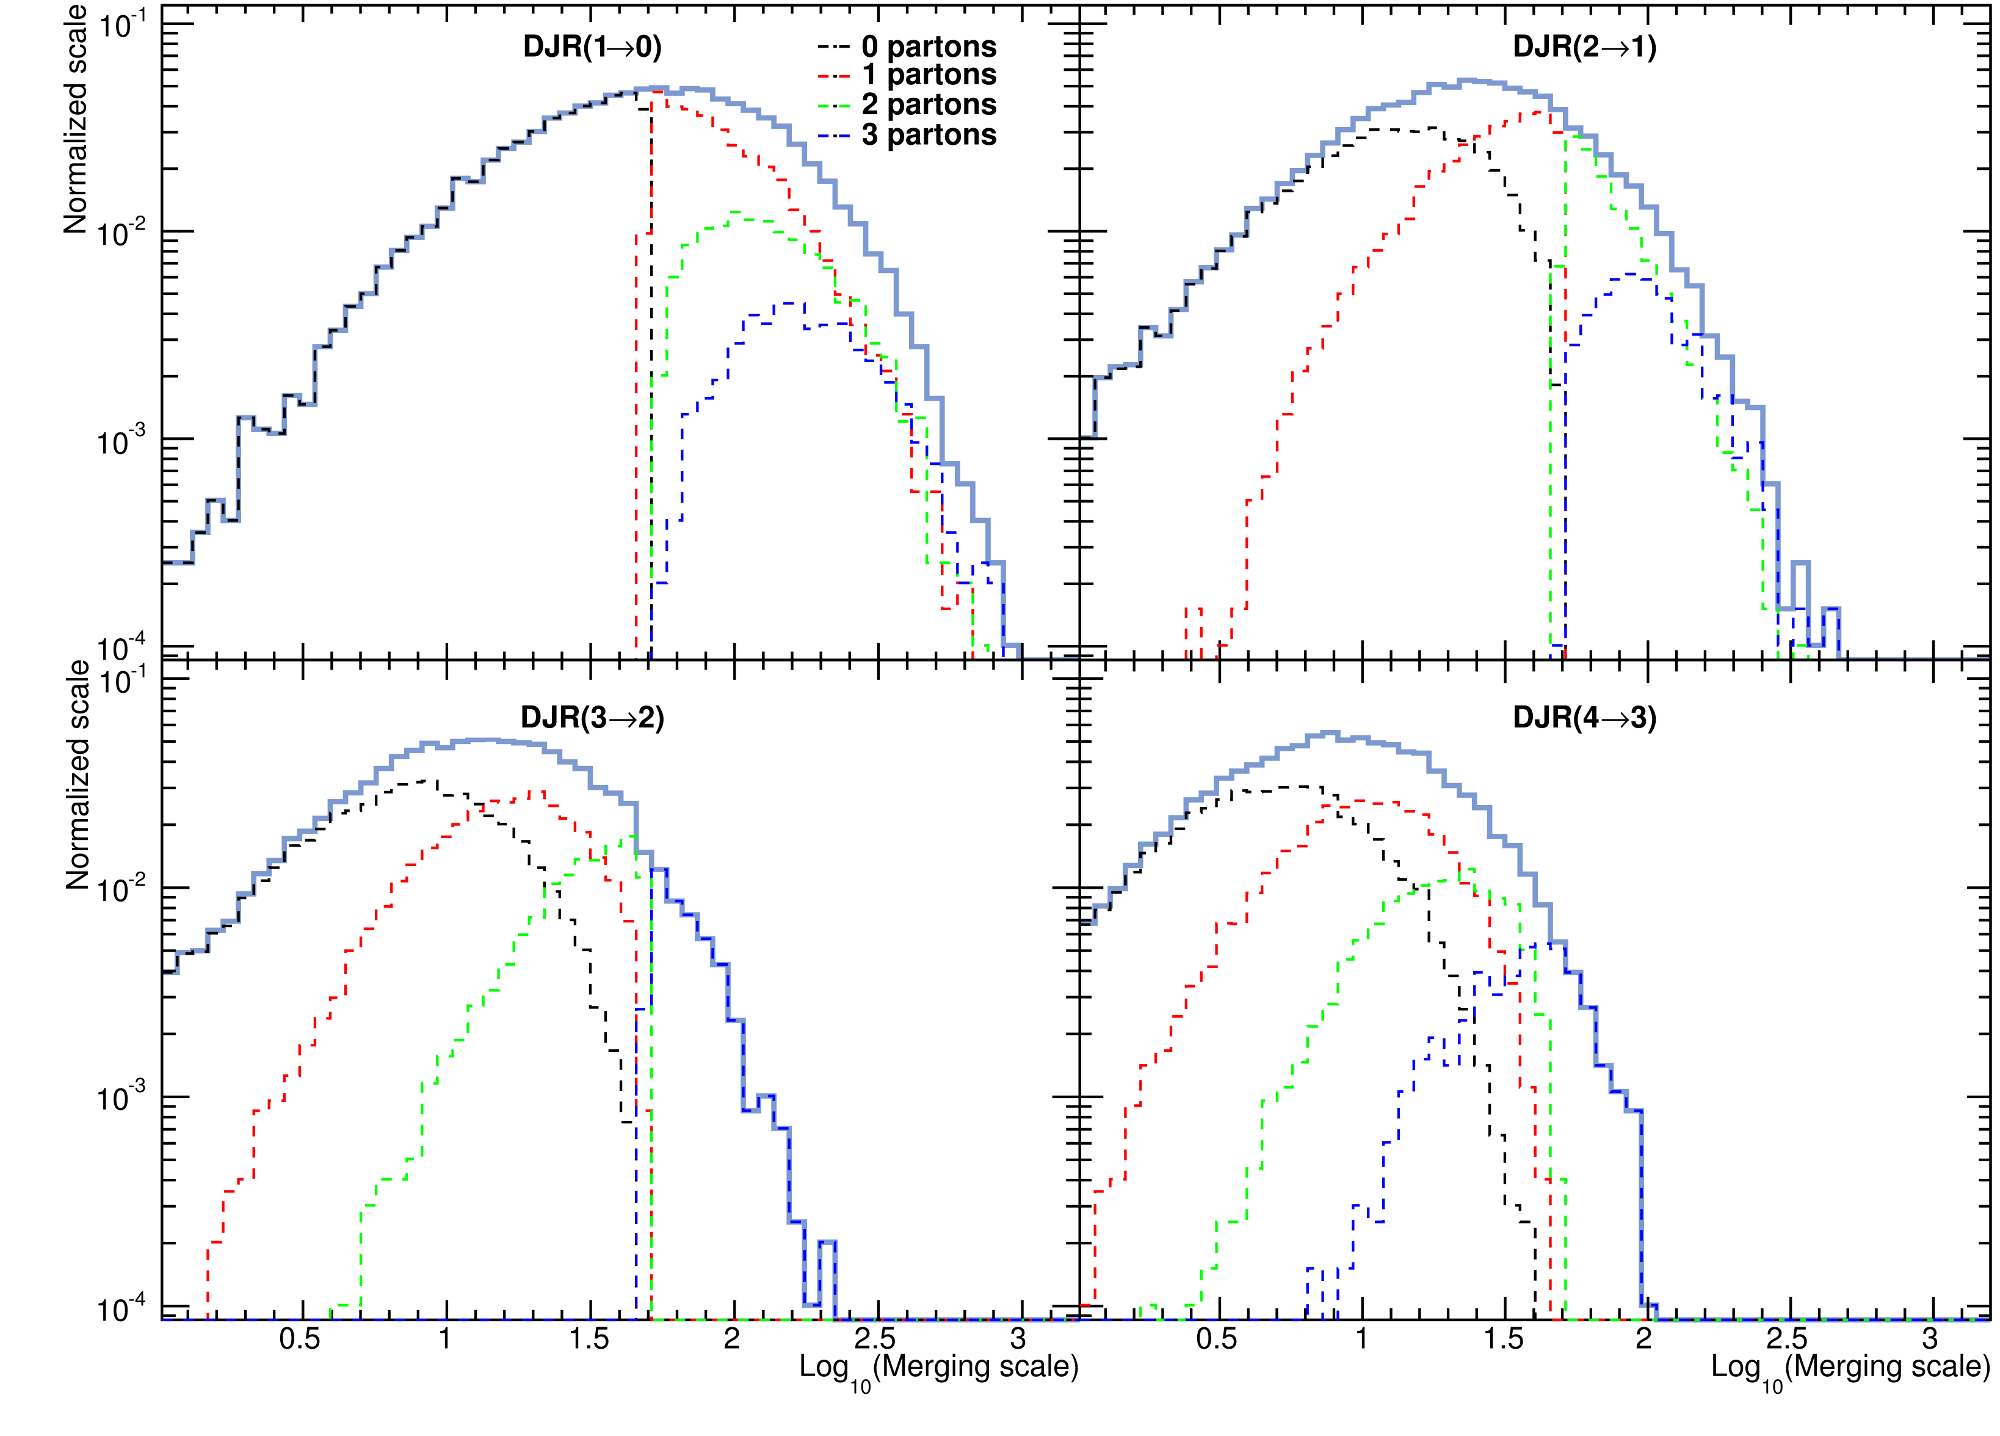
\includegraphics[width=0.5\textwidth]{../figs/DJR_q50_xq20_TTJets13TeV.png}
    %\caption{DJR diagrams for 13 TeV top pair production with $Q_{cut}=100$ GeV and $Q^{X}_{cut}=20$ GeV [optimal case] (top) and $Q_{cut}=60$ GeV and $Q^{X}_{cut}=20$ [non-optimal] (bottom). Bottom figure shows a discontinuity in the transition from 3 to 2 partons at the point where blue-dashed and green-dashed curves meet.}
    %\label{fig:TTJetsMerging}
%  \end{center}
%\end{figure}
%
%\vspace{-.2cm}
%  \begin{block}{}\tiny
%    \textbf{Figure}: DJR diagrams for 13 TeV top pair production with $Q_{cut}=100$ GeV and $Q^{X}_{cut}=20$ GeV [optimal case] (left) and $Q_{cut}=60$ GeV and $Q^{X}_{cut}=20$ [non-optimal] (right). Right figure shows a discontinuity in the transition from 3 to 2 partons at the point where blue-dashed and green-dashed curves meet.
%  \end{block}

\end{frame}


\iffalse
\begin{frame}{CMS: Compact Muon Solenoid}
\vspace{-.2cm}

\begin{columns}
\begin{column}{.30\textwidth}
\begin{block}{}
\begin{itemize}\scriptsize
\item One of two general purpose experiments of LHC
\item Cylinder of 28.7 m long and 15 m height and 14000 tons
\end{itemize}
\tiny{
\begin{equation*}  
\eta = -\text{ln}\left( \text{tan}\left(\frac{\theta}{2}\right)\right)
\end{equation*}
\begin{equation*}
\Delta R=\sqrt{(\Delta\eta)^{2}+(\Delta\phi)^{2}}
\end{equation*}
}%
\end{block}
\end{column}

\begin{column}{.70\textwidth}
\begin{figure}[!Hhtbp]
  \begin{center}
    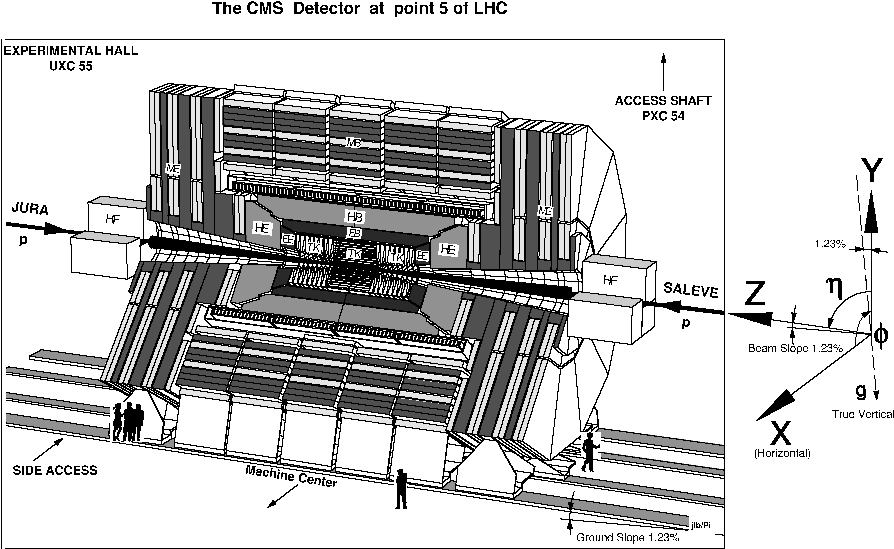
\includegraphics[width=\textwidth]{../figs/CMS_coordinates.jpg}
  \end{center}
\end{figure}
\end{column}
\end{columns}

\vspace{-.2cm}
\begin{block}{}
\begin{itemize}\scriptsize
\item Compact: The calorimeters are inside the magnet
\item Muon: Very precise measurement of muons
\item Solenoid: Solenoidal magnet of 3.8 T magnetic field
\end{itemize}
\end{block}

\end{frame}


\begin{frame}{Sub-detectors}
\vspace{-.2cm}
\begin{figure}[!Hhtbp]
  \begin{center}
    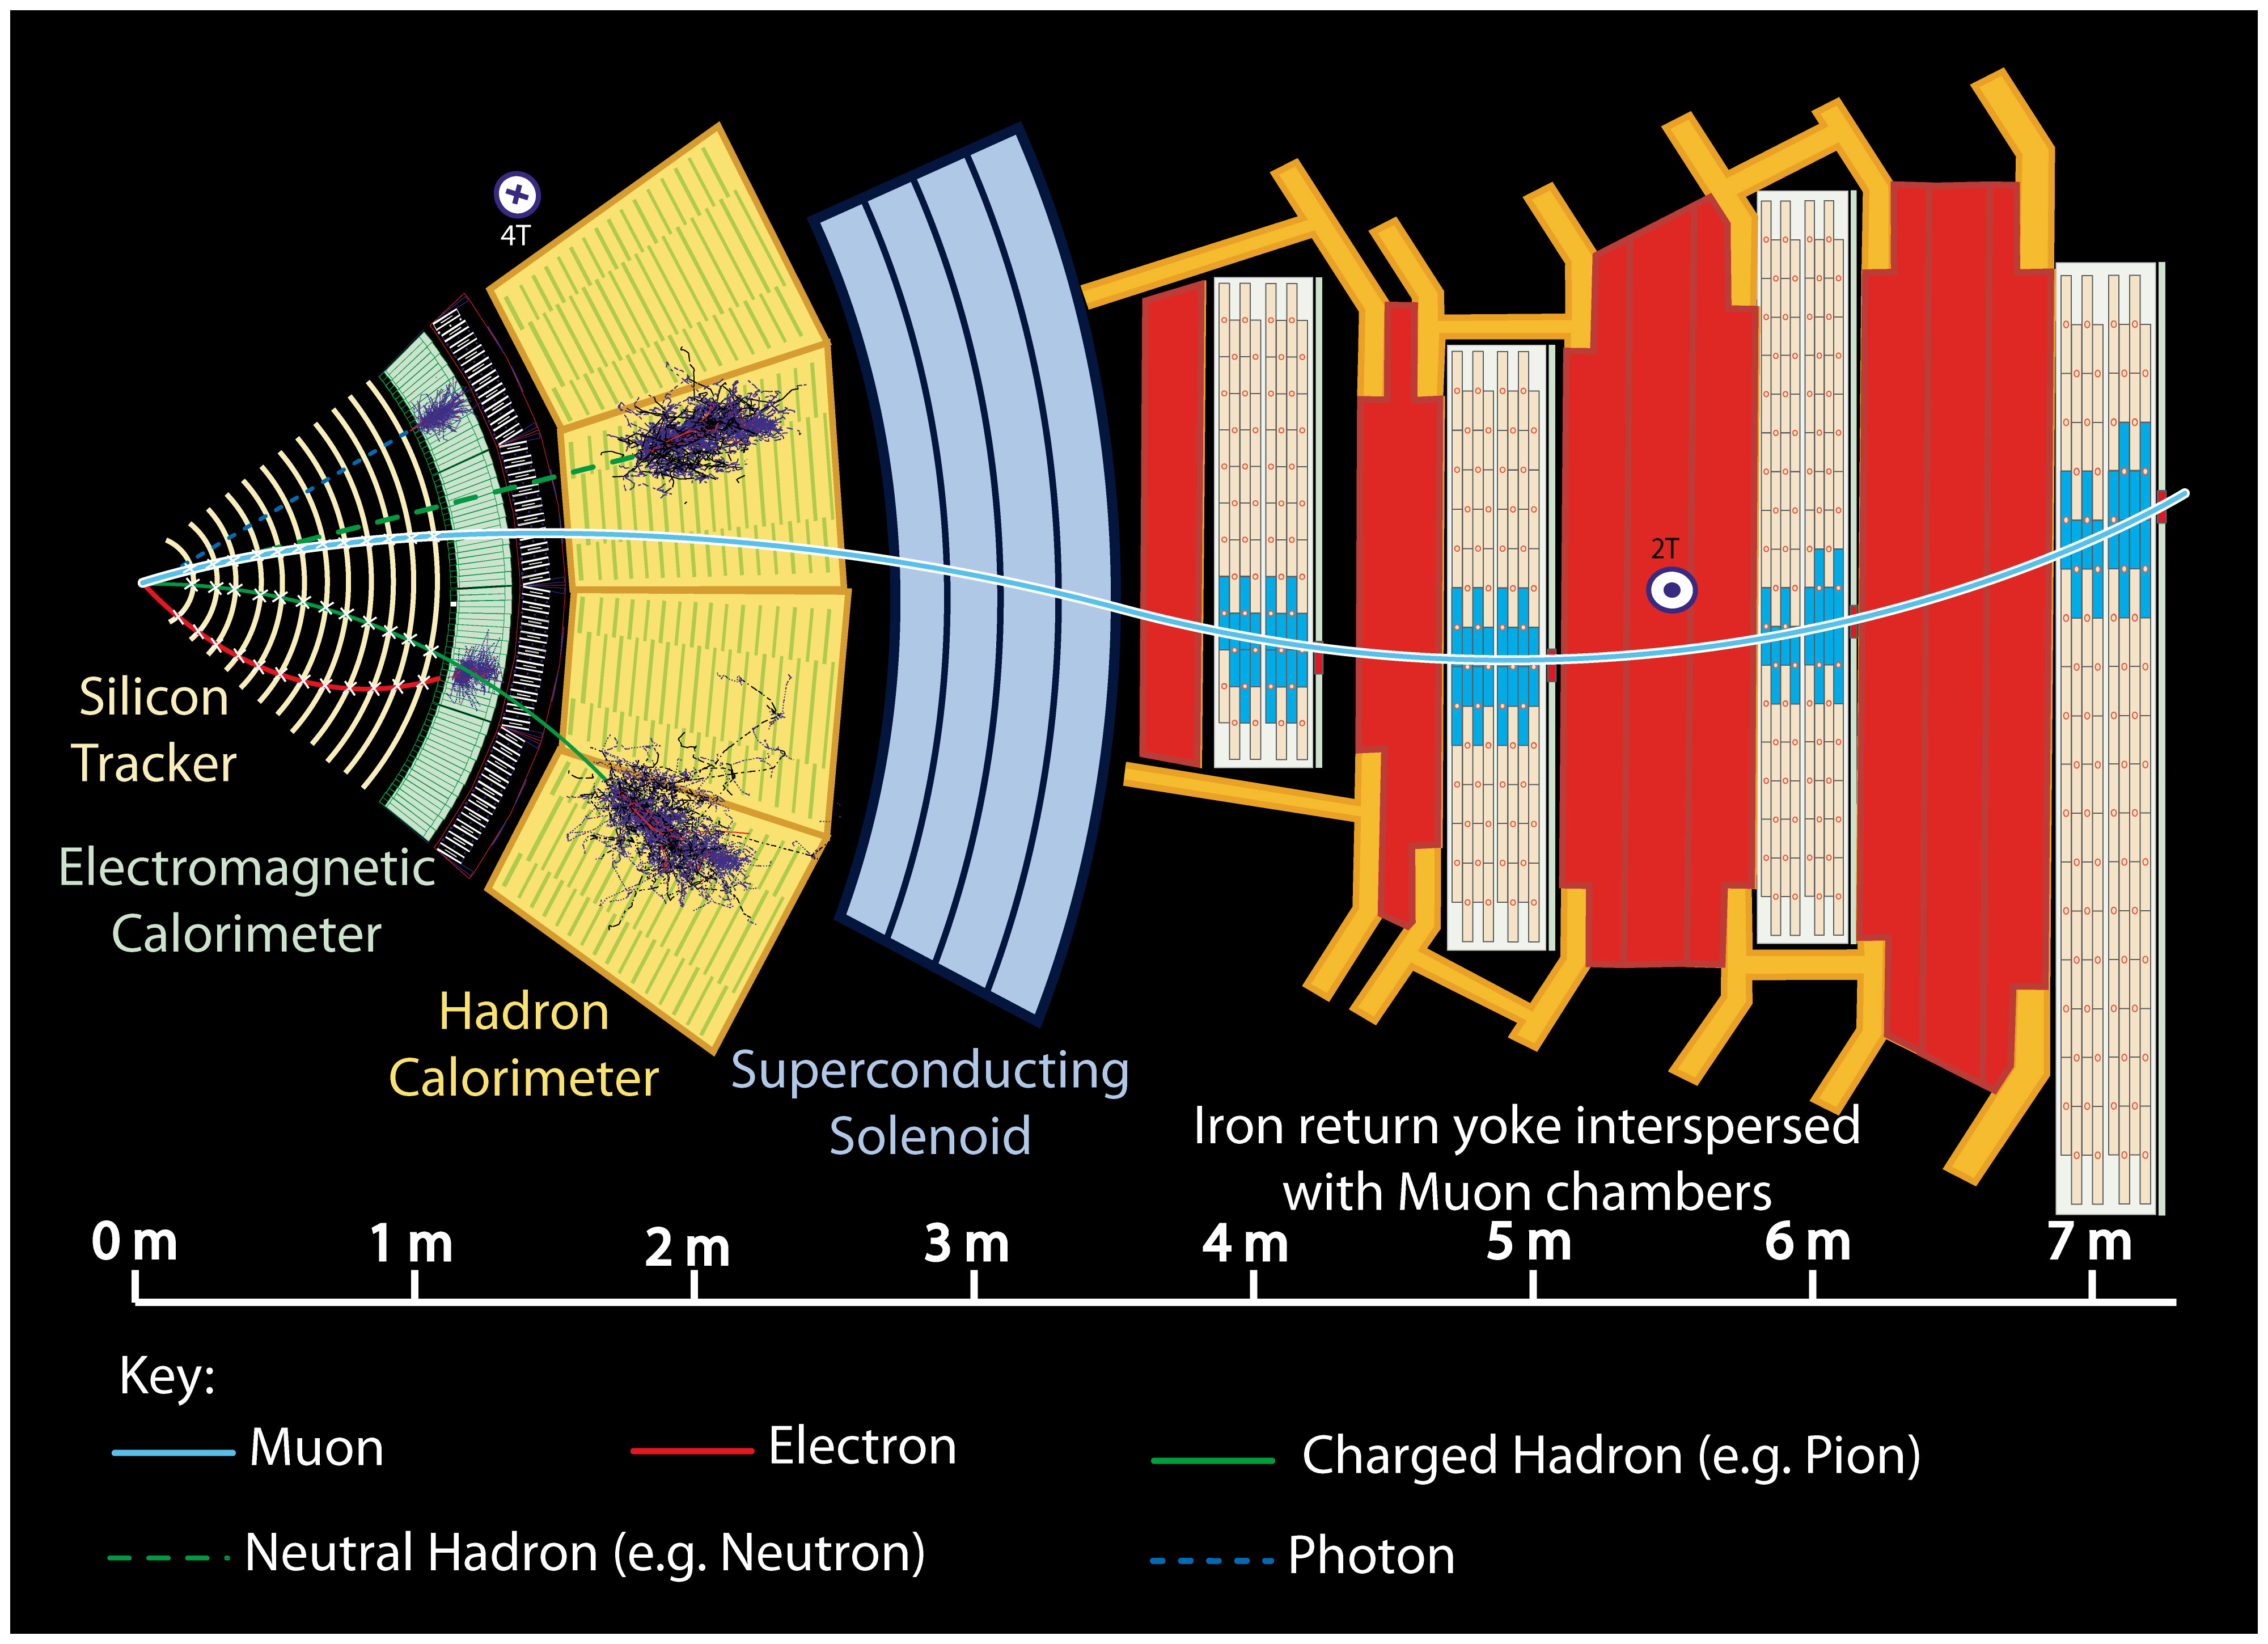
\includegraphics[width=0.7\textwidth]{../figs/PictureforPoint5_oct04_allp.jpg}
    %\caption{CMS sub-detectors and particle identification. }
    %\label{fig:cmsslice}
  \end{center}
\end{figure}
\vspace{-.4cm}
\begin{block}{}
\begin{itemize}\tiny
\item Tracker system: Pixel system (vertex reconstruction) and Silicon strips (Measurement of \pt~of charged particles)
\item Electromagnetic calorimeter (ECAL): 80000 crystals for the measurement of electrons and photons energy
\item Hadron calorimeter (HCAL): Absorber and scintillator to measure the energy of hadrons
\item Muon chambers: RPC, DT and CSC to measure muons \pt
\end{itemize}
\end{block}

\end{frame}


\begin{frame}{Object reconstruction - Jets}
\vspace{-.9cm}

\begin{columns}
\begin{column}{.55\textwidth}
\begin{block}{}
\begin{itemize}\tiny
\item Tracker information is used to reconstruct charged particles $\to$ Charged hadrons, electrons, muons
\item ECAL + HCAL information used to reconstruct the energy of hadrons (neutral and charged)
\item Tracker system + ECAL + HCAL information are combined to reconstruct jets $\to$ objects used to recover the information from a quark or gluon produced in the hard scattering
\item Several algorithms are used to collect all reconstructed particles in a jet: CMS $\to$ anti-kt algorithm with a radius $R=0.5$ (AK5)
\item Jet energy measurement can suffer of missing tracks, pile-up or other detector effects $\to$ Strategies needed to correct jet energy 
\item Jet energy information is analyzed by an MVA algorithm to determine if it was produced by a b quark $\to$ Constrained Secondary Vertex (CSV) discriminator for b-jets in three working points:\\
\tiny{
\textbf{CSVL (Loose)}: Discriminator > 0.244, $\epsilon^{CSVL}_{b}=85$\%, $\epsilon^{CSVL}_{c}=45$\%, $\epsilon^{CSVL}_{l}=10$\%\\
\textbf{CSVM (Medium)}: Discriminator > 0.679, $\epsilon^{CSVM}_{b}=$70\%, $\epsilon^{CSVM}_{c}=$20\%, $\epsilon^{CSVM}_{l}=$1\%\\
\textbf{CSVT (Tight)}: Discriminator > 0.898, $\epsilon^{CSVT}_{b}=50$\%, $\epsilon^{CSVT}_{c}=7$\%, $\epsilon^{CSVT}_{l}=0.2$\%\\
}%
\end{itemize}
\end{block}
\end{column}

\begin{column}{.45\textwidth}
\begin{figure}[!Hhtbp]
\begin{center}
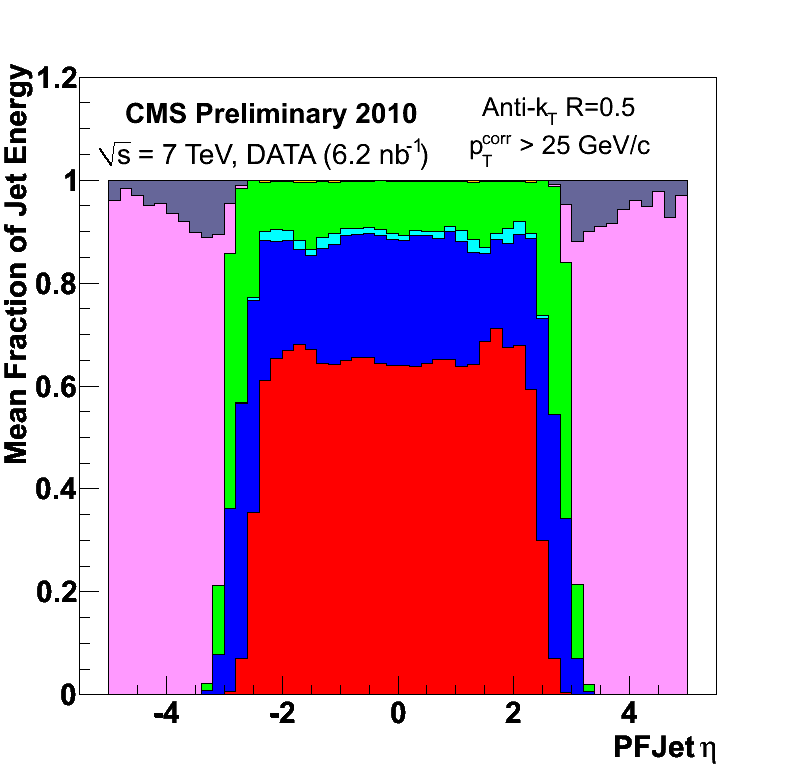
\includegraphics[width=0.6\textwidth,height=0.33\textheight]{../figs/Jet_composition_data_7TeV.png}
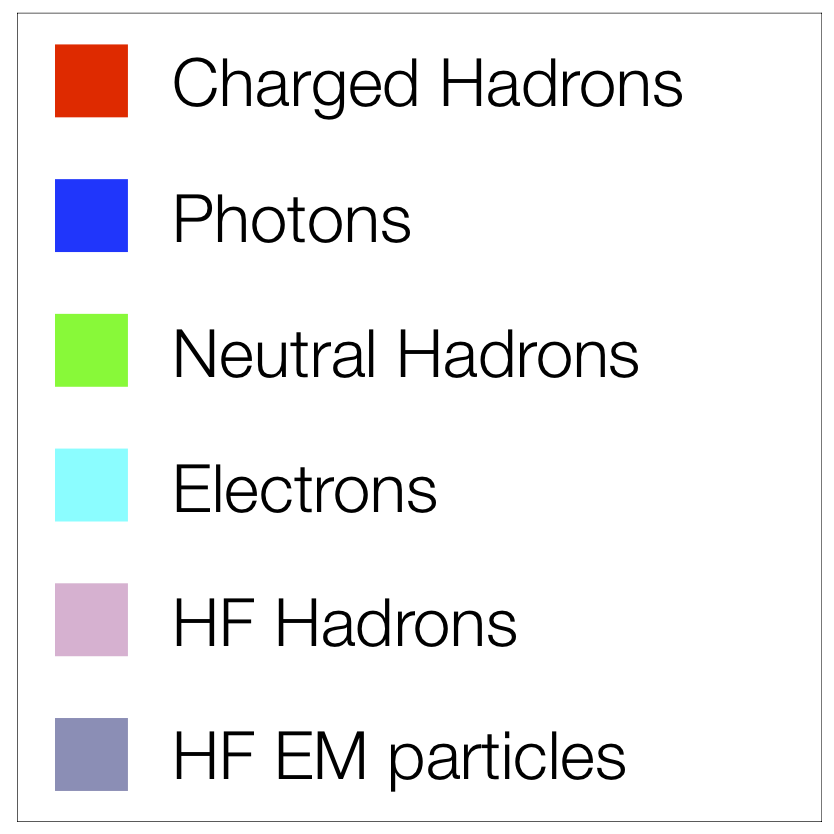
\includegraphics[width=0.3\textwidth]{../figs/Legend_jet_composition.png}\\
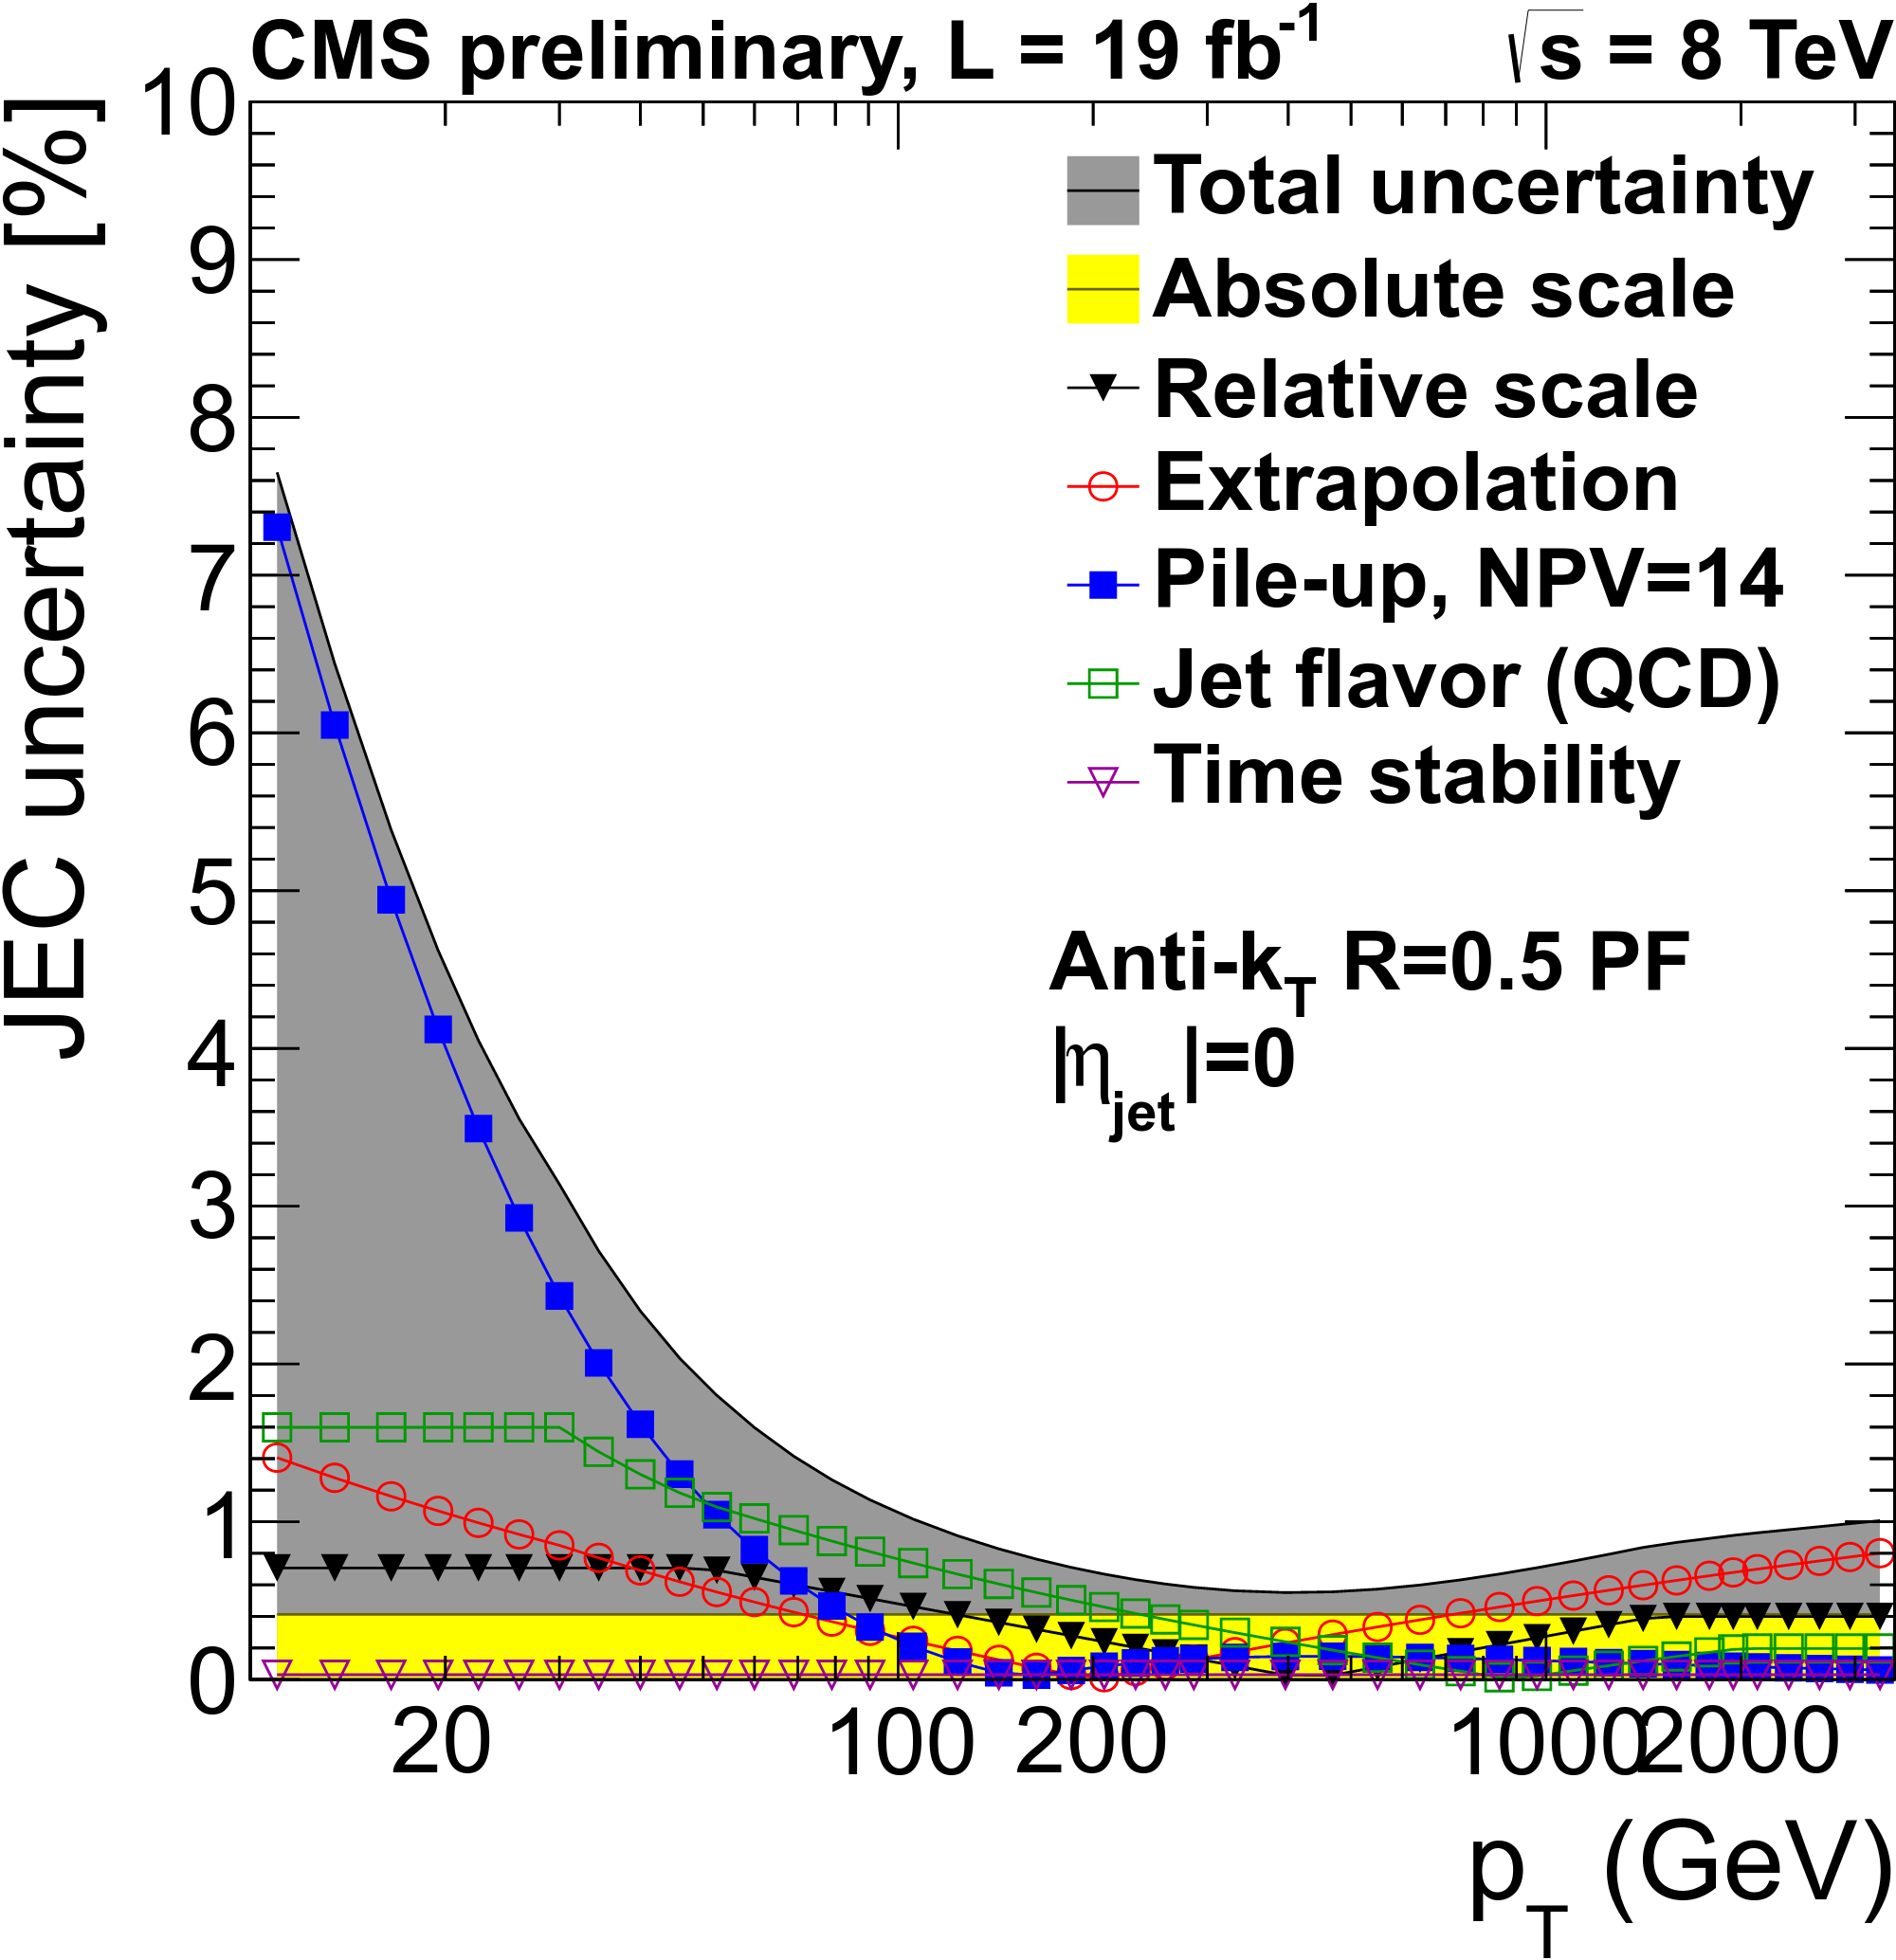
\includegraphics[width=0.55\textwidth,height=0.33\textheight]{../figs/JEC_pt.png}\\
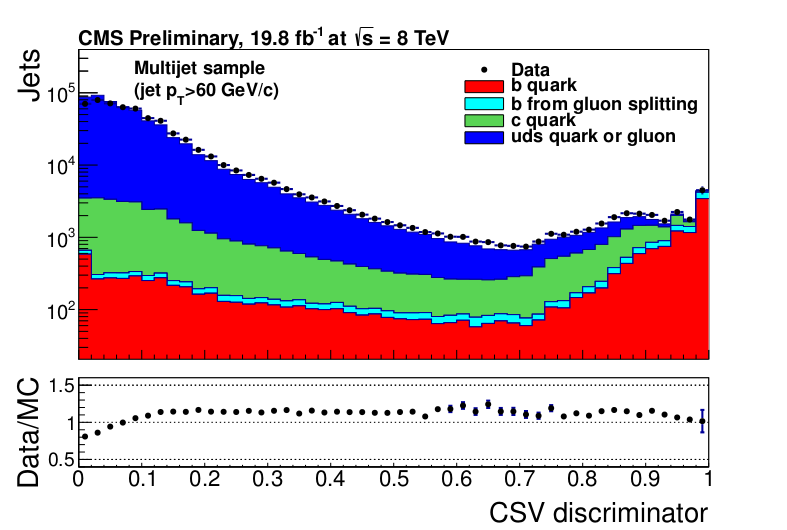
\includegraphics[width=0.6\textwidth,height=0.33\textheight]{../figs/pdf-sub.png}
\end{center}
\end{figure}
\end{column}
\end{columns}

\end{frame}

\fi

%%%%%%%%%%%%%%%%%%%%%%%%%%%%%%%%%%%%%%%%%%%%%%%%%%%%%%%%
%%%%%%%%%%%%%%%%%%%%%%%%%%%%%%%%%%%%%%%%%%%%%%%%%%%%%%%%
\section[Pheno]{Feasibility study for a search of a \Tp~at LHC at 8 TeV}
\setcounter{tocdepth}{2}

\begin{frame}
\begin{center}
Feasibility study for a search of a \Tp~at LHC at 8 TeV
\end{center}
\end{frame}

\subsection{PHENO}

\begin{frame}{Motivation - Samples - Strategy}
\vspace{-.5cm}

\begin{columns}
\begin{column}{.50\textwidth}
\begin{block}{Motivation}
\begin{itemize}\tiny
\item Single produced \Tp~with mixings to light quark generations $\to$ Enhanced production cross section
\item Full hadronic channel:
  \begin{itemize}\tiny
  \item Difficult $\to$ huge backgrounds
  \item Highest number of expected events
  \item It is possible to reconstruct the \Tp~mass
  \item It needs techniques to choose the jets to reconstruct the \Tp
  \end{itemize}
\item $T'\to tH, tZ, bW$ and $Br(T'\to tH)=0.5$ $Br(H\to b\bar{b})=0.57$ $Br(t\to bq\bar{q}')=0.66$
\end{itemize}
\end{block}
\end{column}

\begin{column}{.50\textwidth}
%\begin{table}[htbH]
\begin{center}
\resizebox{\textwidth}{!}{
\begin{tabular}{||l|c|r||}
  \hline\hline
  Process & $\sigma_{\rm 8 TeV}$ (pb) & Expected Events \\ \hline
 Signal ($T'j$) & 0.2 & 700 \\
 \hline
  QCD (bbjjj) & 500 & 10,000,000 \\
  \W+jets & 37,509 & 750,180,000 \\
  \Z+jets & 3,503.71 & 70,074,200 \\
  \ttbar & 234 & 4,680,000 \\
  single-$t$ & 114.85 & 2,297,000 \\
  Di-boson & 96.82 & 1,936,400 \\
  \hline\hline
\end{tabular}
}
%\caption{Cross sections and expected number of events for background processes and signal for a luminosity of 20~$fb^{-1}$. \label{tab:xsec}}
\end{center}
%\end{table}
\vspace{-.5cm}
\begin{block}{}
\tiny $M(5j)$ $\to$ Five jets invariant mass as variable of interest
\end{block}
\end{column}
\end{columns}

\vspace{-.2cm}
\begin{block}{Strategy}
\begin{itemize}\tiny
\item Signal: 3 $b$-quarks and 2 light quarks $\to$ High b-jet multiplicity
\item Real Higgs boson and top quark in signal events
\item Method to have a good identification of the 5 jets coming from the \Tp:
\begin{itemize}\tiny
\item Tag b--jets and keep events with at least two.
\item b-jets pairs used to reconstruct the Higgs boson $\to$ ${\Delta R_{bb} <2.5}$ and pair with closest mass to the Higgs boson mass (125~\GeVcc)
\item b-jets removed from jets collection $\to$ jets pair with closest mass to the W-mass (80~\GeVcc) chosen to reconstruct the \W~boson 
\item Higgs and \W~boson jets removed from jet collection $\to$ the jet giving the closest mass to the top mass (172~\GeVcc), combined with W-jets, was used to reconstruct the top quark
\end{itemize}
\end{itemize}

\end{block}

\end{frame}

\begin{frame}{Selection}
\vspace{-.2cm}

\begin{columns}
\begin{column}{.50\textwidth}
\begin{block}{}
\begin{itemize}\scriptsize
\item \textit{Cut 0}: At least 6 jets with ${p_T > 30}$~GeV/c are required. At least five jets within $|\eta|<2.5$ and at least one jet within $2<|\eta|<5$. The \Tp~decays into five central jets. One associated jet in the forward direction. \\
\textbf{Figure}: $\eta$ distribution of the forward jet produced in association with \Tp. Signal sample is normalized to theoretical cross section and to 20~$fb^{-1}$.
\item \textit{Cut 1}: ${p_{T}(j_{1})>150}$~GeV/c, ${p_{T}(j_{2})>80}$~GeV/c, ${p_{T}(j_{3,4})>60}$~GeV/c
\item \textit{Cut 2}: $H_{T}>630$~GeV/c with $H_{T}=\sum |p_{T}(j)|$\\
\textbf{Figure}: Total hadronic energy for backgrounds (stacked) and signal (over--imposed) normalized to 20~$fb^{-1}$ luminosity. $H_{T}$ is higher in signal than in background events.
\end{itemize}
\end{block}
\end{column}

\begin{column}{.50\textwidth}
\begin{figure}[!Hhtbp]
  \begin{center}
    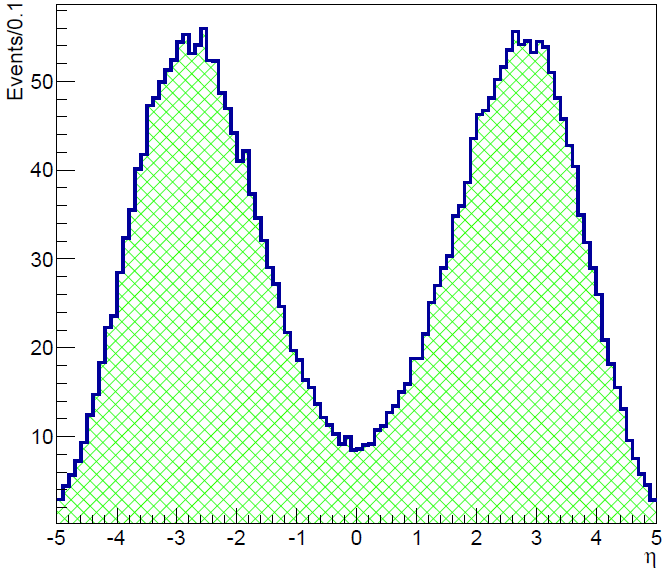
\includegraphics[width=0.75\textwidth]{../figs/Pheno/SixthJet.png}\\
    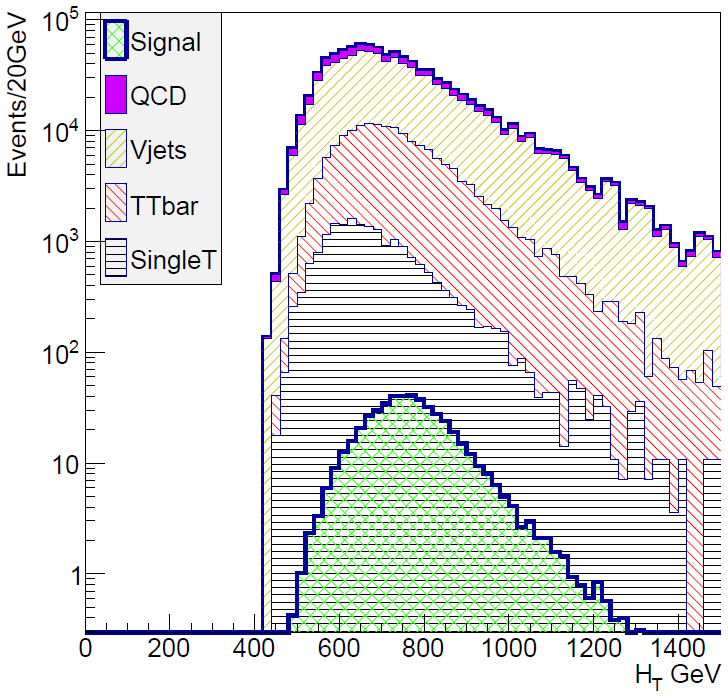
\includegraphics[width=0.75\textwidth]{../figs/Pheno/HT.png}
  \end{center}
\end{figure}
\end{column}
\end{columns}

\end{frame}

\begin{frame}{}
\vspace{-.2cm}

\begin{columns}
\begin{column}{.50\textwidth}
\begin{block}{}
\begin{itemize}\scriptsize
\item \textit{Cut 3}: At least two b-jets with effective CSV algorithm with medium working point
\item \textit{Cut 4}: Events with a Higgs candidate with $p_{T}>200$~GeV/c and a top candidate with $p_{T}>300$~GeV/c\\
\textbf{Figure}: Reconstructed Higgs candidate $p_{T}$ in the x axis and reconstructed top candidate $p_{T}$ in the y axis for backgrounds (left) and signal (right). Signal events have reconstructed Higgs and top with higher \pt~than backgrounds.
\item \textit{Cut 6}: Events with $2.2<\Delta R_{HW}<3.5$ were kept\\
\textbf{Figure}: $\Delta R$ between the reconstructed Higgs and \W~candidates for backgrounds (stacked) and signal (over--imposed) normalized to 20 $fb^{-1}$ luminosity. However signal and backgrounds have a mean value of $\Delta R_{HW}=3$, backgrounds tend to have lower values than signal, as well as larger tails.
\end{itemize}
\end{block}
\end{column}

\begin{column}{.50\textwidth}
\begin{figure}[!Hhtbp]
\begin{center}
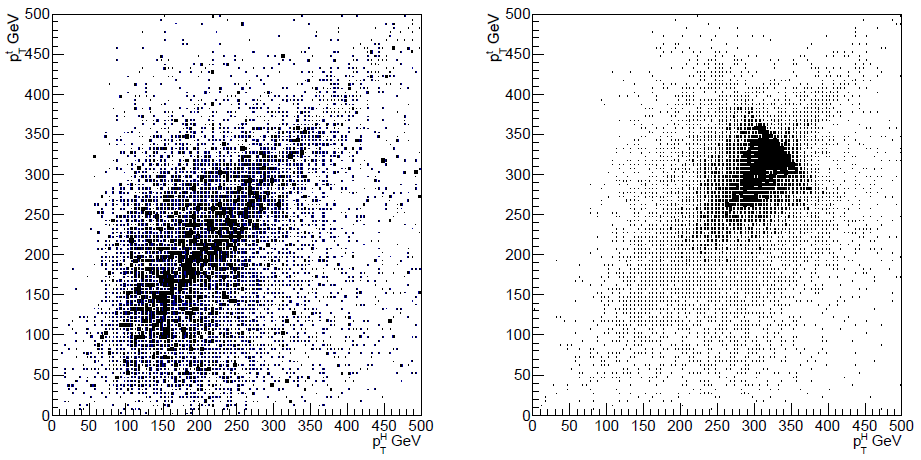
\includegraphics[width=1.0\textwidth]{../figs/Pheno/HPTTPT.png}\\
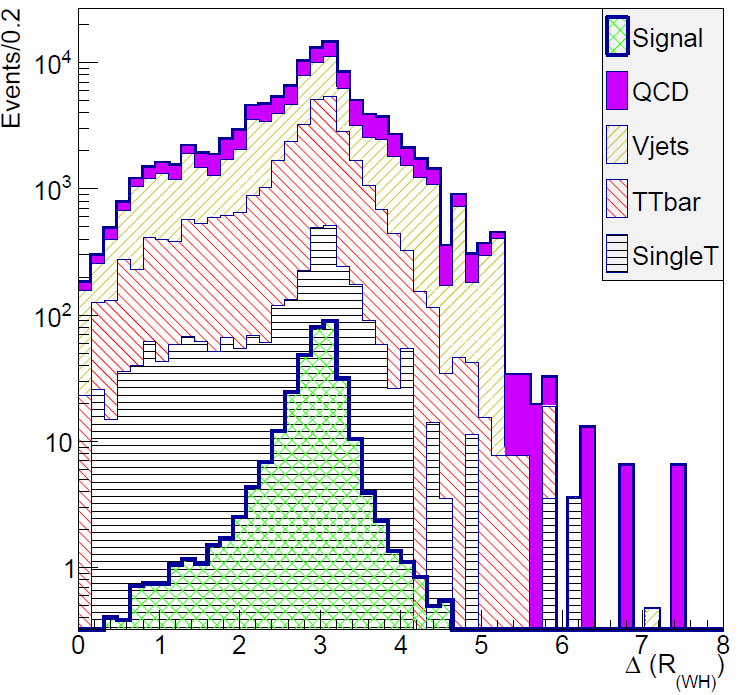
\includegraphics[width=0.75\textwidth]{../figs/Pheno/DRWH.png}
\end{center}
\end{figure}
\end{column}
\end{columns}

\end{frame}

\begin{frame}{}
\vspace{-.2cm}

\begin{columns}
\begin{column}{.50\textwidth}
\begin{block}{}
\begin{itemize}\scriptsize
\item \textit{Cut 7}: Events with $\Delta \phi_{H(bb)}<2.0$ and $\Delta \phi_{top(bW)}<3.3$ were kept
\item \textit{Cut 8}: Events were required to have $\Delta \phi_{W(jj)}<2.3$ 
\item \textit{Cut 9}: Events with a Higgs candidate with a mass between $100$~\GeVcc~and $135$~\GeVcc~were selected\\
\textbf{Figure}: Mass of the reconstructed Higgs candidate for backgrounds (stacked) and signal (over--imposed). Backgrounds have larger tails than signal for the reconstructed Higgs mass.
\item \textit{Cut 10}: Events with $\frac{p_{T}^{H}+p_{T}^{t}}{H_{T}}>0.65$ were kept
\textbf{Figure}: Relative total hadronic energy for backgrounds (stacked) and signal (over--imposed) normalized to 20 $fb^{-1}$ luminosity.
\end{itemize}
\end{block}
\end{column}

\begin{column}{.50\textwidth}
\begin{figure}[!Hhtbp]
  \begin{center}
    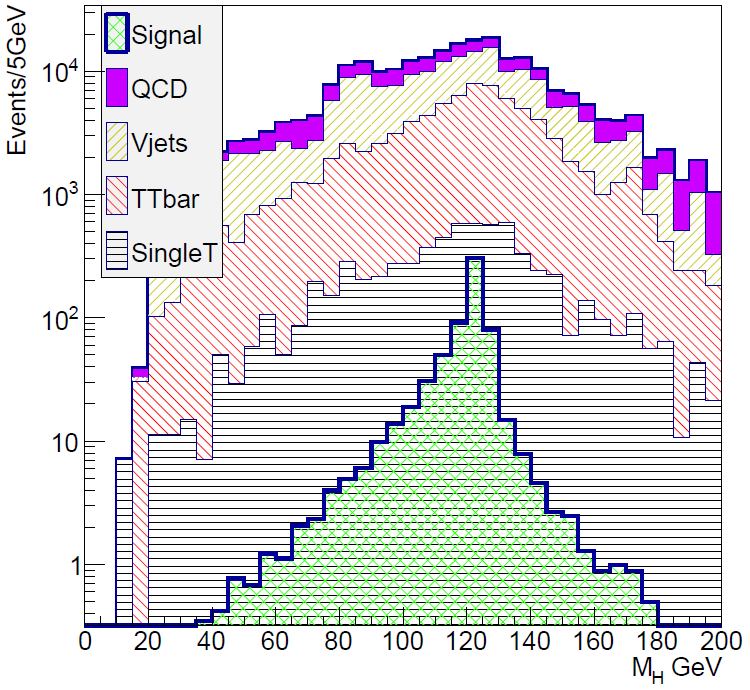
\includegraphics[width=0.75\textwidth]{../figs/Pheno/MH.png}\\
    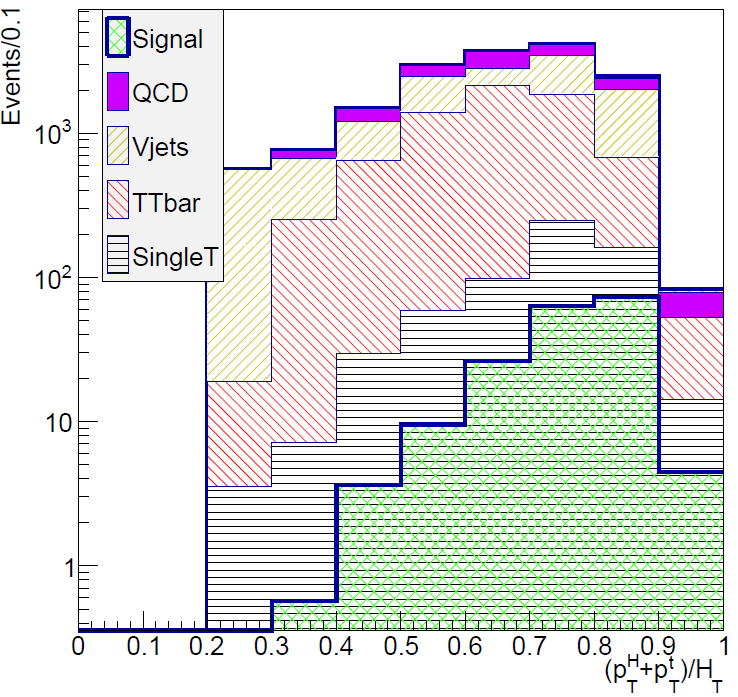
\includegraphics[width=0.75\textwidth]{../figs/Pheno/RelHT.png}
  \end{center}
\end{figure}
\end{column}
\end{columns}

\end{frame}

\begin{frame}{Results}
\vspace{-.2cm}

\begin{columns}
\begin{column}{.50\textwidth}
\begin{block}{}\scriptsize
The number of events falling into a window of $20$~GeV around the \Tp~mass ($M(5j)$) were selected\\
\textbf{Figure}: Reconstructed \Tp~mass after all cuts for backgrounds and signal (stacked) normalized to 20~$fb^{-1}$ luminosity. Signal peak is visible on top of the sum of backgrounds.

\begin{center}
\resizebox{\textwidth}{!}{
\begin{tabular}{l|c|c|c|c}
 & \multicolumn{2}{c|}{unweighted events}  & \multirow{2}{*}{weight} & weighted  \\
 & after Cut 10 & in mass window & & events \\
 \hline
 Signal & $8601$ & $3780$ & $0.018$ &$69 \pm 1$ \\
 \hline
   $t \bar{t}$ & $409$ & $57$ & $7.7$ & $437 \pm 58$ \\
 $W$+jets & $24$ & $3$ & $132$ & $395 \pm 228$ \\
 $QCD$ & $235$ & $34$ & $6.48$ & $220 \pm 38$ \\
 $tW$ & $18$ & $3$ & $11.3$ & $34 \pm 20$ \\
 $t$+ jet & $75$ & $7$ & $3.55$ & $25 \pm 9$ \\
  \hline
  total background & & & & $1112 \pm 352$ \\
\end{tabular}
}
%\caption{Number of signal and background events from utilized MC samples: in the first column the simulated events that pass all kinematic cuts, in the second column the events that fall in the mass window ${710<M_{jjjjj}<750}$~\GeVcc, finally in the fourth column the number of weighted events in the mass window normalized to the physical cross section (the applied weight is listed in the third column). All the errors are statistical only. For the total background, the linear sum of errors was considered.} \label{tab:events}
\end{center}

Discriminators:
\begin{equation*}                                               
\frac{S}{\sqrt{S+B}}=2.0\pm 0.3\, \mbox{and} \, \frac{S}{B}=0.06\pm 0.02                                               
\end{equation*}
\end{block}
\end{column}

\begin{column}{.50\textwidth}
\begin{figure}[!Hhtbp]
  \begin{center}
    \includegraphics[width=1.0\textwidth]{../figs/Pheno/Final.png}
    %\caption{Reconstructed \Tp~mass after all cuts for backgrounds and signal (stacked) normalized to 20~$fb^{-1}$ luminosity. Signal peak is visible on top of the sum of backgrounds.}
    %\label{fig:M5J}
  \end{center}
\end{figure}
\end{column}
\end{columns}

\end{frame}

%\begin{frame}{}
%\vspace{-.2cm}
%
%\begin{columns}
%\begin{column}{.50\textwidth}
%\begin{block}{}
%\begin{itemize}\scriptsize
%\item 
%\end{itemize}
%\end{block}
%\end{column}
%
%\begin{column}{.50\textwidth}
%
%\end{column}
%\end{columns}
%
%\end{frame}


%%%%%%%%%%%%%%%%%%%%%%%%%%%%%%%%%%%%%%%%%%%%%%%%%%%%%%%%
%%%%%%%%%%%%%%%%%%%%%%%%%%%%%%%%%%%%%%%%%%%%%%%%%%%%%%%%
\section[MC]{Monte-Carlo event simulation}
\setcounter{tocdepth}{2}

\begin{frame}
\begin{center}
Monte-Carlo event simulation
\end{center}
\end{frame}

\subsection{Monte-Carlo simulations}
\begin{frame}{Monte-Carlo simulations}
\vspace{-.2cm}
\begin{block}{Central concepts}
\scriptsize \centering{ Usage of random variables and large samplings to calculate mathematical quantities in complex configurations.}\\
In particle physics (referred to LHC) $\to$ Simulation of collisions at three levels:
\begin{itemize}
\item Partonic level: Scattering of partons inside protons.
\item Hadronic level: Showering and hadronization of collision products.
\item Detector level: Simulation of the detector response to the particles generated in a collision.
\end{itemize}
\end{block}

\begin{figure}[!Hhtbp]
  \begin{center}
    \includegraphics[width=0.3\textwidth]{../figs/Tchannel_T_single.jpg}
    \includegraphics[width=0.35\textwidth]{Hadronization.png}
    \includegraphics[width=0.3\textwidth]{detector_part.png}
  \end{center}
\end{figure}

\end{frame}


\begin{frame}{Parton simulation}
\vspace{-.2cm}

\begin{columns}
\begin{column}{.50\textwidth}
  \begin{block}{}\tiny
    \begin{itemize}
    \item Model proposed to understand collisions of non-fundamental particles.
    \item Valence quarks of a proton are the $u$ and $d$
    \item Sea: $b$, $c$ or $s$ quarks and gluons
    \item Parton distribution function: $f\equiv f(x,Q^{2})$ is the number density of a given quark or gluon as a function of the resolution scale $Q^{2}$ and the fraction of momentum carried by the parton $x$
    \item Simulation done up to a perturbative level: Tree-level or Leading order (LO), one loop or Next-to-Leading-Order (NLO), two loops or Next-to-Next-to-Leading-Order (NNLO), ...
    \end{itemize}
  \end{block}
\vspace{-.3cm}
\begin{block}{}\tiny
\textbf{Tool}: MadGraph $\to$ Matrix-element generator for event generation, calculation of LO cross sections and particle widths. This tool is specially interesting for implementations of BSM models.
\end{block}
\vspace{-.3cm}
\begin{block}{}\tiny
\textbf{Figure}: Martin-Stirling-Thorne-Watt proton PDF for $Q^{2}= 10\, \text{GeV}^{2}$ [left] and $Q^{2}= 10^{4}\, \text{GeV}^{2}$ [right]. $x$ is the fraction of momentum carried by the parton and $f(x,Q^{2})$ the PDF function.
\end{block}
\vspace{-.3cm}
\begin{block}{}\tiny
\textbf{Equation}: $f_{i,j}$ corresponds to the PDF's of the initial partons, $\mathcal{M}_{ij\rightarrow lm}$ is the matrix element of the process
\end{block}
\end{column}

\begin{column}{.50\textwidth}
\begin{figure}[!Hhtbp]
  \begin{center}
    \includegraphics[width=1.0\textwidth]{../figs/mstw2008nlo68cl_allpdfs.jpg}
    %\caption{Martin-Stirling-Thorne-Watt proton PDF for $Q^{2}= 10\, \text{GeV}^{2}$ [left] and $Q^{2}= 10^{4}\, \text{GeV}^{2}$ [right]. $x$ is the fraction of momentum carried by the parton and $f(x,Q^{2})$ the PDF function.}
    %\label{fig:MSTW}
  \end{center}
\end{figure}
\vspace{-.2cm}
{\tiny
\begin{eqnarray}
  %\label{eq:DiffXS}
d\sigma_{ij\rightarrow lm} & = & \left( \int_{0}^{1}\int_{0}^{1}f_{i}(x_{i},Q^{2})f_{j}(x_{j},Q^{2})dx_{i}dx_{j} \right) \nonumber \\
  & \times & \frac{d^{3}p_{l}}{(2\pi)^{2}2E_{l}}\frac{d^{3}p_{m}}{(2\pi)^{2}2E_{m}} \nonumber \\
  & \times & \delta^{4}\left( p_{i}+p_{j}-p_{l}-p_{m} \right) \nonumber \\
  & \times & |\mathcal{M}_{ij\rightarrow lm}|^{2} \nonumber                                     
\end{eqnarray}
}%

\end{column}

\end{columns}
\end{frame}


\begin{frame}{Hadron and Detector simulation}
\vspace{-.2cm}

\begin{columns}
\begin{column}{.50\textwidth}
  \begin{block}{Hadron simulation}\scriptsize
    \begin{itemize}
    \item Quarks produced from hard interaction $\to$ not seen freely due to strong interaction.
    \item Two processes simulations:
      \begin{itemize}\scriptsize
      \item Showering: radiation from initial or final states.
      \item Hadronization: formation of hadrons from final state quarks and gluons.
      \end{itemize}
    \item Hadronization simulation generates the ``soft'' part of the event. Parton simulation generates the hard (interaction) part.
    \end{itemize}
  \end{block}
\vspace{-.3cm}
\begin{block}{}\tiny
\textbf{Tool}: Pythia $\to$ it could take the events produced by a matrix-element generator. If it hadronizes partonic level events, a special procedure (merging) for the interface between the two generations must be done to assure ``physical'' simulations. If not, it generates directly the hadrons from the hard interaction.
\end{block}
\end{column}

\begin{column}{.50\textwidth}
  \begin{block}{Detector simulation}\scriptsize
    \begin{itemize}
    \item Simulation of the detector response to particles simulated in the collision (after hadronization).
    \item Detailed simulation of the detector: subdetectors, cells, layers, electronic cards, ...
    \item It is done as close as possible to reality, however some real detector problems. Two possibilities to solve remaining issues:
      \begin{itemize}\scriptsize
      \item Generate run-dependent MC simulations
      \item Apply corrections to generic MC simulations, to get closer to data.
      \end{itemize}
    \end{itemize}
  \end{block}
\vspace{-.3cm}
\begin{block}{}\tiny
\textbf{Tool}: GEANT 4 $\to$ CMS private detector simulation, with all details of the detector. DELPHES $\to$ Tool to simulate a generic detector with the main pieces: tracking system embedded in a magnetic field, calorimeters and muon system.
\end{block}

\end{column}

\end{columns}
\end{frame}


\begin{frame}{Parton simulation}
\vspace{-.2cm}

\begin{columns}
\begin{column}{.50\textwidth}
  \begin{block}{}
    \tiny \centering 
  \end{block}
\end{column}

\begin{column}{.50\textwidth}

\end{column}

\end{columns}
\end{frame}

%%%%%%%%%%%%%%%%%%%%%%%%%%%%%%%%%%%%%%%%%%%%%%%%%%%%%%%%
%%%%%%%%%%%%%%%%%%%%%%%%%%%%%%%%%%%%%%%%%%%%%%%%%%%%%%%%
\section[Analysis]{Search for a single produced \Tp~decaying into top and Higgs in the full hadronic final state}
\setcounter{tocdepth}{2}

\begin{frame}
\begin{center}
Search for a single produced \Tp~decaying into top and Higgs in the full hadronic final state
\end{center}
\end{frame}


\subsection{Introduction - Analysis Strategy}
\begin{frame}{Introduction - Analysis Strategy}
\vspace{-.2cm}
\begin{columns}

\begin{column}{.50\textwidth}
\begin{block}{}
\begin{itemize}\scriptsize
\item Single produced \Tp~with an associated jet
\item Full hadronic final state: \\ $T'\to t H \to b W^{+} \bar{b} b \to b \bar{b} j j b$
\item Reconstruction of \Tp~mass: $M(5j)$
\item Main challenges:
  \begin{itemize}\scriptsize
  \item Huge backgrounds $\rightarrow$ Mainly QCD and \ttbar
  \item \Tp~reconstruction with high jet multiplicity
  \end{itemize}
\item Fundamental tools for background discrimination:
  \begin{itemize}\scriptsize
  \item B-tagged jets multiplicity
  \item \Tp~reconstruction procedure
  \end{itemize}
\end{itemize}
\end{block}
\end{column}

\begin{column}{.50\textwidth}
\begin{center}
\includegraphics[width=0.9\textwidth]{../figs/Tchannel_T_single.jpg}\\
\includegraphics[width=1.0\textwidth]{../figs/pheno_prod_single_tp.png}
\end{center}
\end{column}
\end{columns}

\end{frame}

\begin{frame}{Datasets}
\vspace{-.2cm}

%\begin{table*}[htbH]
\begin{center}
\resizebox{\textwidth}{!}{
\begin{tabular}{|c|c|}
\hline 
Dataset name & Int. Luminosity ($\text{pb}^{-1}$) \\
\hline
/MultiJet/Run2012A-22Jan2013-v1/AOD & 889.4 \\
/MultiJet1Parked/Run2012B-05Nov2012-v2/AOD & 4429.0 \\
/MultiJet1Parked/Run2012C-part1-05Nov2012-v2/AOD & 494.6 \\
/MultiJet1Parked/Run2012C-part2-05Nov2012-v2/AOD & 6654.0 \\
/MultiJet1Parked/Run2012D-part1-10Dec2012-v1/AOD & 5955.1 \\
/MultiJet1Parked/Run2012D-part2-17Jan2013-v1/AOD & 734.0 \\
/MultiJet1Parked/Run2012D-part2-PixelRecover-17Jan2013-v1 & 538.4 \\
\hline
\multicolumn{1}{|r|}{\textit{Total}} & 19694.5 \\
\hline
\end{tabular}
}
%\caption{List of Multijet Primary Dataset used in the analysis and the corresponding integrated luminosity calculated using the golden JSON (Java Script Object Notation) file. The golden JSON file contains the information about the luminosity sections considered as good for all runs. A good luminosity section is defined as a luminosity section where the detector was fully functioning, this is all subsystems were taking data and without problems.  \label{tab:datasets}}
\end{center}
%\end{table*}

%\begin{table*}[htbH]
\begin{center}
\resizebox{\textwidth}{!}{
\begin{tabular}{|c|c|c|}
\hline 
Samples & Cross-Section (pb) & Number of events\\
\hline
QCD\_Pt-120to170\_TuneZ2star\_8TeV\_pythia6 & 16\(\times 10^4\) & 5.9M\\
QCD\_Pt-170to300\_TuneZ2star\_8TeV\_pythia6 & 34\(\times 10^3\) & 5.8M\\
QCD\_Pt-300to470\_TuneZ2star\_8TeV\_pythia6 & 18\(\times 10^2\) & 5.9M\\ 
QCD\_Pt-470to600\_TuneZ2star\_8TeV\_pythia6 & 114 & 3.9M\\
QCD\_Pt-600to800\_TuneZ2star\_8TeV\_pythia6 & 27 & 3.9M\\
QCD\_Pt-800to1000\_TuneZ2star\_8TeV\_pythia6 & 3.5 & 3.9M\\
QCD\_HT-500To1000\_TuneZ2star\_8TeV-madgraph-pythia6 & 84\(\times 10^2\) & 30M\\ 
QCD\_HT-1000ToInf\_TuneZ2star\_8TeV-madgraph-pythia6 & 2\(\times 10^2\) & 14M\\ 
TTJets\_MSDecays\_central\_TuneZ2star\_8TeV-madgraph-tauola & 247.7 [NNLO] & 62M\\
TprimeJetToTH\_\textbf{M-700}\_TuneZ2star\_8TeV-madgraph\_tauola & 143.7 & 99K \\
\hline
\end{tabular}
}
%\caption{List of Monte-Carlo background samples used in the analysis, their corresponding cross-section and their number of events.\label{tab:MCbkg}}
\end{center}
%\end{table*}

\tiny{Signal samples were done with $T'\to tH$ with $H\to\tau^{+}\tau^{-}$ (6\%) and $H\to b\bar{b}$ (94\%). Correction with weight of 0.61 to obtain correct $Br(H\to b\bar{b})=0.57$. }

\end{frame}

\begin{frame}{Event selection}
\vspace{-.2cm}

\begin{columns}

\begin{column}{.55\textwidth}
\begin{block}{Event processing}
\begin{itemize}\scriptsize
  \item Data processed using ``golden'' JSON file: Consider only validated lumi sections
  \item PAT processing
    \begin{itemize}\tiny
    \item Jets reconstructed with PF algorithm and CHS
    \item Jets: \ptg{20} and $|\eta|<5$
    \item At least one good primary vertex: $\text{n.d.o.f.} \ge 4,\; |z|<24 \;\text{cm},\; |\rho|< 2 \;\text{cm}$
    \item Global tag: Calibration and alignment info for data, MC corrected to get close to data conditions
    \end{itemize}
  \item Pile-up corrections: Simulated PU in MC was corrected to observed PU in Data
\end{itemize}
\end{block}
\end{column}

\begin{column}{.45\textwidth}
\vspace{-.9cm}
\begin{figure}[!Hhtbp]
  \begin{center}
    \includegraphics[width=1.0\textwidth]{../figs/Ana/Nvtcs.png}
  \end{center}
\end{figure}
\vspace{-.75cm}
\begin{block}{}
\tiny Number of vertices distribution for data and MC samples. The comparison has been performed after basic selection except number of b-tagged jets (the basic selection is described in the next slides). The gray band correspond to the statistical error of MC samples sum. Normalization of MC samples was done to the 19.7~fb$^{-1}$.
\end{block}
\end{column}

\end{columns}
\end{frame}

\begin{frame}{Basic selection}
\vspace{-.2cm}

\begin{block}{}
  \begin{itemize}\scriptsize
  \item Trigger L1: at least 4 central jets (\etal{3}) with \ptg{32}~or \ptg{36}~or \ptg{40} \\
                    or at least 2 central jets with \ptg{52}~or \ptg{56}~or \ptg{64} \\
                    or events with \HTg{125}~or \HTg{150}~or \HTg{175}
  \item HLT: 6 central jets with a \ptg{20}, 4 with a \ptg{60} and 2 with a \ptg{80}
  \item \textbf{First offline cut}: 2 jets with \ptg{90}, 2 jets with \ptg{70} and 2 jets with \ptg{30}
  \end{itemize}
\end{block}

\begin{columns}
\begin{column}{.50\textwidth}
\vspace{-.2cm}
\begin{block}{}
  \scriptsize \textbf{Second cut}: At least 5 jets with \ptg{30} and \etal{2.5} and at least one additional jet with \ptg{30} and \etal{5} were required
\end{block}

\vspace{-.2cm}
\begin{block}{}
\scriptsize \textbf{Figure}: Distribution of pseudorapidity of the accompanying jet produced with the \Tp. The distribution is taken from the signal MC sample with M=700 \GeVcc~and it is normalized to unity.
\end{block}
\end{column}

\begin{column}{.50\textwidth}
\vspace{-.2cm}
\begin{figure}[!Hhtbp]
  \begin{center}
    \includegraphics[width=1.0\textwidth]{../figs/Ana/SixthJetMCTruth.png}
    %\caption{Distribution of pseudorapidity of the accompanying jet produced with the \Tp. The distribution is taken from the signal MC sample with M=700 \GeVcc~and it is normalized to unity.}
    %\label{fig:SixthJetTp}
  \end{center}
\end{figure}
\end{column}
\end{columns}

\end{frame}

\begin{frame}{}
\vspace{-.2cm}

\begin{columns}
\begin{column}{.50\textwidth}
\begin{block}{}
\scriptsize \textbf{3rd cut}: the leading jet was required to have a \ptg{150}
\end{block}
\vspace{-.2cm}
\begin{block}{}
\scriptsize \textbf{4th cut}: \HTg{550} was required
\end{block}
\vspace{-.2cm}
\begin{block}{}
\scriptsize \textbf{Figure}: Distribution of the $H_{T}$ variable for data and the sum of the MC samples normalized to luminosity. The signal sample (M=700 \GeVcc) is over-imposed on top of the stack of the MC samples. The gray band represents the statistical uncertainties from the sum of the MC background. Reasonable agreement is observed, with the multijet process as the dominant process at this stage. Normalization of samples was done to luminosity.
\end{block}
\end{column}

\begin{column}{.50\textwidth}
\begin{figure}[!Hhtbp]
  \begin{center}
    \includegraphics[width=1.0\textwidth]{../figs/Ana/HT.png}
    %\caption{Distribution of the $H_{T}$ variable for data and the sum of the MC samples normalized to luminosity. The signal sample (M=700 \GeVcc) is over-imposed on top of the stack of the MC samples. The gray band represents the statistical uncertainties from the sum of the MC background. Reasonable agreement is observed, with the multijet process as the dominant process at this stage. Normalization of samples was done to luminosity.}
    %\label{fig:HT}
  \end{center}
\end{figure}
\end{column}

\end{columns}
\end{frame}

\begin{frame}{}
\vspace{-.2cm}

\begin{columns}
\begin{column}{.50\textwidth}
\begin{block}{}
\scriptsize \textbf{B-tagging}: CSV (Constrained Secondary Vertex) algorithm $\to$ Multivariate technique that give a discriminator indicating how likely a jet is coming from a b-quark
\textbf{Working points}: Loose, Medium and Tight\\\tiny{CSVL$\to$0.244 \\$\epsilon^{CSVL}_{b}=85$\%, $\epsilon^{CSVL}_{c}=45$\%, $\epsilon^{CSVL}_{l}=10$\% \\CSVM$\to$0.679\\ $\epsilon^{CSVM}_{b}=$70\%, $\epsilon^{CSVM}_{c}=$20\%, $\epsilon^{CSVM}_{l}=$1\% \\CSVT$\to$0.898\\ $\epsilon^{CSVT}_{b}=50$\%, $\epsilon^{CSVT}_{c}=7$\%, $\epsilon^{CSVT}_{l}=0.2$\%}
\end{block}
\vspace{-.2cm}
\begin{block}{}
\scriptsize \textbf{5th cut}: at least 3 CSVM b-tagged jets. Only jets with $|\eta|<=2.4$ considered for b-tagging.
\end{block}
\vspace{-.2cm}
\begin{block}{}
\scriptsize \textbf{Figure}: B-tagged CSVM jet multiplicity for data and MC samples before requiring at least 3 CSVM b-tagged jets. The sum of MC samples is normalized to the integrated luminosity.
\end{block}
\end{column}

\begin{column}{.50\textwidth}
\begin{figure}[!Hhtbp]
  \begin{center}
    \includegraphics[width=1.0\textwidth]{../figs/Ana/NCSVM.png}
    %\caption{B-tagged CSVM jet multiplicity for data and MC samples before requiring at least 3 CSVM b-tagged jets. The sum of MC samples is normalized to the integrated luminosity.}
    %\label{fig:Nb}
  \end{center}
\end{figure}
\end{column}

\end{columns}
\end{frame}



\begin{frame}{Corrections to MC for b-tagging}
\vspace{-.2cm}

\begin{columns}
\begin{column}{.50\textwidth}
\begin{block}{}
\scriptsize Scale factors derived from data/MC comparisons $\to$ $SF^{flavor}_{\eta}(p_{T})$\\
As mean values: $SF^{b\; or\; c}\sim 0.94$ and $SF^{light}\sim 1.06$
\end{block}
\vspace{-.2cm}
\begin{block}{}
\scriptsize In order to apply the SF's a weight per event is calculated\\
$w=\frac{P(\text{DATA})}{P(\text{MC})}$ with \\ \tiny{
$P(\text{MC}) = \prod_{i=\text{tagged}} \varepsilon_i \prod_{j=\text{not tagged}} (1-\varepsilon_j)$\\
$P(\text{DATA}) = \prod_{i=\text{tagged}} \text{SF}_i \varepsilon_i \prod_{j=\text{not tagged}} (1-\text{SF}_j \varepsilon_j)$ \\
}
\end{block}
\vspace{-.2cm}
\begin{block}{}
\tiny B-tagging efficiencies defined as\\
$\varepsilon_f(i,j) = \frac{N_f^\text{b-tagged}(i,j)}{N_f^\text{Total}(i,j)}$ where \\
where $ N_f^\text{Total}(i,j) $ and $ N_f^\text{b-tagged}(i,j) $ are the total number and the number of b-tagged jets, respectively, of flavor $ f $ in the $ (p_\text{T},\eta) $ bin $ (i,j) $ for a given MC sample.
\end{block}
\vspace{-.2cm}
\begin{block}{}
\scriptsize \textbf{Figure}: Distribution of the weights from b-tagging scale factors for all MC samples.
\end{block}
\end{column}

\begin{column}{.50\textwidth}
\begin{figure}[!Hhtbp]
  \begin{center}
    \includegraphics[width=1.0\textwidth]{../figs/Ana/SF_weight.png}
    %\caption{Distribution of the weights from b-tagging scale factors for all MC samples.}
    %\label{fig:SFweight}
  \end{center}
\end{figure}
\end{column}

\end{columns}
\end{frame}

\begin{frame}{\Tp~reconstruction with a $\chi^{2}$ sorting algorithm}
\vspace{-.2cm}
\scriptsize

\begin{itemize}
\item $\chi^{2}$ sorting algorithm used to identify the \Tp~decay products and to reconstruct the Higgs and top candidates
\item $\chi^{2}$ variable defined for each jets combination in an event
\item The combination that minimizes this variable gives the best fit of the objects under reconstruction
\end{itemize}

\begin{equation*}
\chi^{2}=\frac{(M_{H}-M_{bb})^{2}}{\sigma_{H}^{2}}+\frac{(M_{W}-M_{jj})^{2}}{\sigma_{W}^{2}}+\frac{(M_{t}-M_{bjj})^{2}}{\sigma_{t}^{2}}
%\label{eq:chi2def}
\end{equation*}

\begin{itemize}
\item $M_{H}=125$~\GeVcc, $M_{W}=84.06$~\GeVcc, $M_{t}=175.16$~\GeVcc, $\sigma_{H}=12.4$~\GeVcc, and $\sigma_{W}=10.12$~\GeVcc~and $\sigma_{t}=17.35$~\GeVcc. From similar MC studies.
\item For the Higgs reconstruction only CSVM b-tagged jets were considered
\item For the \W~reconstruction all jets with a \ptg{30} were considered
\item For the top reconstruction one b-tagged jet and the pair of jets used for the \W~were utilized
\end{itemize}

\end{frame}

\begin{frame}{}
\vspace{-.2cm}

\begin{columns}
\begin{column}{.50\textwidth}

\begin{figure}[!Hhtbp]
  \begin{center}
    \includegraphics[width=1.0\textwidth]{../figs/Ana/Exclusive_Efficiency_V8.png}
    %\includegraphics[width=0.46\textwidth]{figs/Ana/Inclusive_Efficiency_V8.png}
    %\caption{Reconstruction efficiency by the $\chi^{2}$ algorithm of the Higgs boson, \W~boson, top quark and \Tp, as the ratio of the number of events where the particle was correctly reconstructed to the number of events where jets could be matched to partons [left] and to the total number of events [right]}
    %\label{fig:RecEff}
  \end{center}
\end{figure}

\vspace{-.2cm}
\begin{block}{}
\scriptsize \textbf{Figure}: Reconstruction efficiency by the $\chi^{2}$ algorithm of the Higgs boson, \W~boson, top quark and \Tp, as the ratio of the number of events where the particle was correctly reconstructed to the number of events where jets could be matched to partons.
\end{block}
\end{column}

\begin{column}{.50\textwidth}

\begin{figure}[!Hhtbp]
  \begin{center}
    \includegraphics[width=1.0\textwidth]{../figs/Ana/HundresdsMassChi2Tp.png}
    %\includegraphics[width=0.45\textwidth]{figs/Ana/FiftiesMassChi2Tp.png}
    %\caption{Reconstructed \Tp~mass for all mass points from the $\chi^{2}$ sorting algorithm after basic selection. Each mass point is normalized to luminosity and its corresponding cross section. A gaussian fit of these distributions will be presented afterward in section~\ref{sec:finalsel}, accompanied with a discussion about the resolution on the reconstruction of the \Tp.}
    %\label{fig:RecT}
  \end{center}
\end{figure}

\vspace{-.2cm}
\begin{block}{}
\scriptsize \textbf{Figure}: Reconstructed \Tp~mass for some mass points from the $\chi^{2}$ sorting algorithm after basic selection. Each mass point is normalized to luminosity and its corresponding cross section.
\end{block}
\end{column}

\end{columns}
\end{frame}

\begin{frame}{Selection based on reconstructed objects}
\vspace{-.2cm}
\scriptsize

\begin{columns}
\begin{column}{.50\textwidth}
\vspace{-.2cm}
\begin{block}{}
\tiny
\begin{itemize}
\item Selection optimized via a multidimensional scan of variables 
\item Signal discrimination evaluated by $S/B$, using as signal the $M=700$\GeVcc~mass point, and as background the \ttbar~and QCD\_HT-500To1000
\item Selection has been adjusted to keep at least 10 signal events, for the 700~\GeVcc~mass point, after the full selection
\item \textbf{Data/MC plots are shown for illustration, but final background estimation is derived from data}
\end{itemize}
\end{block}
\vspace{-.2cm}
\begin{block}{}
\scriptsize \textbf{1st criterion}: $\chi^{2}<8$
\end{block}
\vspace{-.2cm}
\begin{block}{}
\scriptsize \textbf{Figure}: Distribution of the $\chi^{2}$ variable for data and MC samples. The signal sample used has a \Tp~mass of 700 \GeVcc. Backgrounds present higher values than the signal. The sum of MC is normalized to the integrated luminosity.
\end{block}
\end{column}

\begin{column}{.50\textwidth}
\begin{figure}[!Hhtbp]
  \begin{center}
    \includegraphics[width=1.0\textwidth]{../figs/Ana/chi2Nm1.png}
    %\caption{Distribution of the $\chi^{2}$ variable for data and MC samples. The signal sample used has a \Tp~mass of 700 \GeVcc. Backgrounds present higher values than the signal. The sum of MC is normalized to the integrated luminosity. }
    %\label{fig:chi2}
  \end{center}
\end{figure}
\end{column}

\end{columns}

\end{frame}

\begin{frame}{}
\vspace{-.2cm}
    \begin{block}{}\scriptsize
      \textbf{2nd criterion}: $\Delta R(bb)<1.2$\\
      \textbf{3rd criterion}: Higgs candidate mass between 105 and 145 \GeVcc
    \end{block}

\vspace{-.5cm}
\begin{columns}
\begin{column}{.50\textwidth}
\begin{figure}[!Hhtbp]
  \begin{center}
    \includegraphics[width=0.9\textwidth]{../figs/Ana/DRbbNm1.png}
  \end{center}
\end{figure}

\vspace{-.7cm}
    \begin{block}{}\tiny
      $\Delta R$ of the 2 b-tagged jets used to reconstruct the Higgs candidate after $\chi^{2}$ cut.
    \end{block}
\end{column}

\begin{column}{.50\textwidth}
\begin{figure}[!Hhtbp]
  \begin{center}
    \includegraphics[width=0.9\textwidth]{../figs/Ana/HMNm1.png}
  \end{center}
\end{figure}

\vspace{-.7cm}
    \begin{block}{}\tiny
      Distribution for $M(H_{cand})$ for data and the sum of Monte Carlo samples. All others selection criteria are applied up to this one.
    \end{block}
\end{column}

\end{columns}

\end{frame}


\begin{frame}{}
\vspace{-.2cm}
    \begin{block}{}\scriptsize
      \textbf{4th criterion}: $(M(top^{2nd})+M(W^{2nd}))/M(H)>6.8$\\
      \textbf{5th criterion}: $\Delta R (T' j^{6})>4.8$\\
      \textbf{6th criterion}: $H_{T}>0.67$
    \end{block}

\vspace{-.5cm}
\begin{columns}
\begin{column}{.50\textwidth}
\begin{figure}[!Hhtbp]
  \begin{center}
    \includegraphics[width=0.8\textwidth]{../figs/Ana/M2HPNm1.png}
  \end{center}
\end{figure}

\vspace{-.7cm}
    \begin{block}{}\tiny
      Distribution of $(M(top^{2nd})+M(W^{2nd}))/M(H)$ for data and the sum of the Monte Carlo samples. Selection criteria are applied up to Higgs mass cut. The low statistics in the multijet (QCD) MC sample is visible at this stage.
    \end{block}
\end{column}

\begin{column}{.50\textwidth}
\begin{figure}[!Hhtbp]
  \begin{center}
    \includegraphics[width=0.8\textwidth]{../figs/Ana/DRTp6JNm1.png}
  \end{center}
\end{figure}

\vspace{-.7cm}
    \begin{block}{}\tiny
      Distributions for $\Delta R (T' j^{6})$  for data and the sum of Monte Carlo samples. All others criteria are applied up to this one. The low statistics in the multijet (QCD) MC sample is visible at this stage.
    \end{block}
\end{column}

\end{columns}

\end{frame}

\begin{frame}{Selection optimization}
\vspace{-.2cm}

\begin{table}[htbH]
\begin{center}
\resizebox{\textwidth}{!}{
\begin{tabular}{|c|c|c|}
\hline 
Cut & $S/B$ & $S/\sqrt{S+B}$ \\
\hline
$\chi^{2}<8$ & $3.4\ex{-2} \pm 2.85\ex{-3}$  & $ 0.96 \pm 0.05$  \\
$\Delta R(bb)<1.2$ & $4.76\ex{-2} \pm 4.52\ex{-3}$ & $1.10 \pm 0.07$  \\
%$1.6<\Delta R (W_{cand} H_{cand})<4.0$ & $4.82\ex{-2} \pm 4.59\ex{-3}$  & $1.10 \pm 0.07$  \\
$105$ \GeVcc~$< M(H_{cand}) < 145$ \GeVcc~& $6.37\ex{-2} \pm 6.74\ex{-3}$  & $1.22 \pm 0.08$  \\
$(M(top^{2nd})+M(W^{2nd}))/M(H_{cand})>6.8$ & $0.15 \pm 0.03$  & $1.45 \pm 0.16$  \\
$\Delta R (T j^{6})>4.8$ & $0.42 \pm 0.19$  & $1.67 \pm 0.32$  \\
Relative $H_{T}>0.67$ & $1.16 \pm 0.17$  & $2.13 \pm 0.17$  \\
\hline
\end{tabular}
%\caption{$S/B$ and $S/\sqrt{S+B}$ from MC samples for each step of the selection after reconstruction of resonances with the $\chi^{2}$ sorting algorithm. Only $M=700$ \GeVcc~signal, \ttbar~and QCD\_HT-500To1000 MC samples were used. \label{tab:Estimators}}
}
\end{center}
\end{table}

\vspace{-.2cm}
    \begin{block}{}\scriptsize
      $S/B$ and $S/\sqrt{S+B}$ from MC samples for each step of the selection after reconstruction of resonances with the $\chi^{2}$ sorting algorithm. Only $M=700$ \GeVcc~signal, \ttbar~and QCD\_HT-500To1000 MC samples were used.
    \end{block}

\end{frame}

\begin{frame}{Trigger efficiency}
\vspace{-.2cm}

\begin{columns}
\begin{column}{.50\textwidth}
   \begin{block}{}\scriptsize
     \begin{itemize}
     \item Prescaled trigger requiring \HTg{400} as reference.
     \item The \pt~of the 6th leading jet has been used to parametrize the trigger efficiency.
     \item Efficiency = number of events passing analysis and reference triggers / number of events passing only HLT\_HT400
     \end{itemize}
    \end{block}

\vspace{-.2cm}
    \begin{block}{}\tiny
      \textbf{Figure}: Efficiency in data and the MC signal samples for events passing trigger bit HLT\_Dijet80\_Dijet60\_Dijet20 with respect to trigger bit HLT\_HT400 after full selection. This efficiency is parametrized as function of the 6$^{th}$ jet $p_{T}$. The dispersion observed is about 10\% between data and signal MC samples, while only about 4\%  for \ttbar. Efficiencies for signal MC samples with \Tp~masses equal to 600, 700, 800, 900 and 1000~\GeVcc~are shown with \ttbar~and data.
    \end{block}
\end{column}

\begin{column}{.50\textwidth}
\begin{figure}[!Hhtbp]
  \begin{center}
    \includegraphics[width=1.0\textwidth]{../figs/Ana/Trigger_Eff_hundreds_FullSel.png}
    %\includegraphics[width=0.45\textwidth]{../figs/Ana/Trigger_Eff_fifties_FullSel.png}
    %\caption{Efficiency in data and the MC signal samples for events passing trigger bit HLT\_Dijet80\_Dijet60\_Dijet20 with respect to trigger bit HLT\_HT400 after full selection. This efficiency is parametrized as function of the 6$^{th}$ jet $p_{T}$. The dispersion observed is about 10\% between data and signal MC samples, while only about 4\%  for \ttbar. This efficiency is parametrized as function of the 6$^{th}$ jet $p_{T}$. Efficiencies for signal MC samples with \Tp~masses equal to 600, 700, 800, 900 and 1000~\GeVcc~are shown with \ttbar~and data [left]. Efficiencies for signal MC samples with \Tp~masses equal to 650, 750, 850 and 950~\GeVcc~are shown with \ttbar~and data [right].}
    \label{fig:TrigEffPostMH}
  \end{center}
\end{figure}
\end{column}

\end{columns}


\end{frame}


%%%%%%%%%%%%%%%%%%%%%%%%%%%%%%%%%%%%%%%%%%%%%%%%%%%%%%%%
%%%%%%%%%%%%%%%%%%%%%%%%%%%%%%%%%%%%%%%%%%%%%%%%%%%%%%%%
\section[Conclusion]{Conclusions, perspectives}
\subsection{Conclusions}
\begin{frame}{Conclusions}
\vspace{-.5cm}
\begin{block}{}
\begin{itemize}\scriptsize
  \item Feasibility study for a search of a \Tp~at LHC at 8 TeV
  %\begin{itemize}\scriptsize
  %  \item Design of an strategy for a search of a \Tp~in the single production mode in the full hadronic final state at 8 TeV LHC run.
    \begin{itemize}\tiny
      \item Les Houches 2013: Physics at TeV Colliders: New Physics Working Group Report \\arXiv:1405.1617
      \item Fully hadronic decays of a singly produced vectorlike top partner at the LHC \\Phys.Rev. D90 (2014) 11, 115008
    \end{itemize}
  %\end{itemize}
  \item MC simulations studies
    \begin{itemize}\scriptsize
      \item MadGraph
        \begin{itemize}\tiny
          \item Validation of releases to enter the CMS MC simulation central production
          \item Several scripts written and updated for collaboration usage
          \item Users support
        \end{itemize}
      \item Pythia 8
        \begin{itemize}\tiny
          \item Comparison of MadGraph + Pythia 8 simulation with other generators and data using RIVET
        \end{itemize}
      \item MadSpin        
        \begin{itemize}\tiny
          \item Inclusion of MadSpin for the gridpack generation of \ttbar~in CMS central production
        \end{itemize}
    \end{itemize}
  \item Search for a single produced \Tp~decaying into top and Higgs in the full hadronic final state
\end{itemize}
\end{block}
\end{frame}

\subsection{Perspectives}
\begin{frame}{Perspectives}
\vspace{-.3cm}
\begin{block}{}
\begin{itemize}\scriptsize
  \item Étude des désintégrations radiatives $Z^0\to\mu\mu\gamma$
  \begin{itemize}\scriptsize
    \item Échelle d'énergie pour 
    \item Finaliser l'étude des incertitudes systématiques
  \end{itemize}
  \item Recherche du boson de Higgs du Modèle Standard dans le canal $H\to\gamma\gamma$
  \begin{itemize}\scriptsize
    \item Réoptimisation de la classification utilisée
    \item Observation d'un excès dans le canal diphoton, excès observé dans d'autres canaux (et dans ATLAS) : découverte d'un nouveau boson, compatible avec un boson de Higgs du Modèle Standard
    \item Propriétés de l'excès (spin, couplages, ...) ? Découverte dans le canal $H\to\gamma\gamma$ seul ?
  \end{itemize}
  \item Production associée d'un boson de Higgs dans le canal $h\to\gamma\gamma$ dans le cadre d'un modèle de quarks vecteurs
  \begin{itemize}\scriptsize
    \item Étude prospective en simulation complète
    \item Étude sur les données récoltées à 
  \end{itemize}
\end{itemize}
\end{block}
\vspace{-.1cm}

\begin{block}{}
\begin{itemize}\scriptsize
\item L'analyse porte sur les données 2011 et 2012 et a été rendue publique le 4 juillet dernier. La quantité de données a doublé depuis... et le LHC continue à accumuler des données !
\item Longue période d'arrêt du LHC pour 2013-2014... avant reprise des collisions à 
% \item Caractérisation de la nouvelle particule
\end{itemize}
\end{block}
\end{frame}

\begin{frame}
\vspace{-.5cm}
\begin{center}
Observation of a new boson at a mass of 125 GeV\\with the CMS experiment at the LHC
\\\tiny
PLB 716 (2012) 30-61 - CMS-PAS-HIG-12-020 - arXiv:1207.7235
\end{center}
%\begin{center}
%\includegraphics[width=.4\textwidth]{plots/Higgs/HIG-12-028/fig16.pdf}
%\includegraphics[width=.4\textwidth]{plots/Higgs/HIG-12-028/fig18.pdf}
%\\
%\includegraphics[width=.4\textwidth]{plots/Higgs/HIG-12-028/fig17.pdf}
%\includegraphics[width=.4\textwidth]{plots/Higgs/HIG-12-028/fig19.pdf}
%\end{center}
\vspace{-.8cm}
\begin{center}
Merci de votre attention !
\end{center}
\end{frame}

%%%%%%%%%%%%%%%%%%%%%%%%%%%%%%%%%%%%%%%%%%%%%%%%%%%%%%%%
%%%%%%% BACKUP
%%%%%%%%%%%%%%%%%%%%%%%%%%%%%%%%%%%%%%%%%%%%%%%%%%%%%%%%
\appendix
\section{BACKUP}
\begin{frame}
\begin{center}
\LARGE
BACKUP
\end{center}
\end{frame}

\begin{frame}
\tableofcontents
\end{frame}



\end{document}